\documentclass[]{book}
\usepackage{lmodern}
\usepackage{amssymb,amsmath}
\usepackage{ifxetex,ifluatex}
\usepackage{fixltx2e} % provides \textsubscript
\ifnum 0\ifxetex 1\fi\ifluatex 1\fi=0 % if pdftex
  \usepackage[T1]{fontenc}
  \usepackage[utf8]{inputenc}
\else % if luatex or xelatex
  \ifxetex
    \usepackage{mathspec}
  \else
    \usepackage{fontspec}
  \fi
  \defaultfontfeatures{Ligatures=TeX,Scale=MatchLowercase}
\fi
% use upquote if available, for straight quotes in verbatim environments
\IfFileExists{upquote.sty}{\usepackage{upquote}}{}
% use microtype if available
\IfFileExists{microtype.sty}{%
\usepackage{microtype}
\UseMicrotypeSet[protrusion]{basicmath} % disable protrusion for tt fonts
}{}
\usepackage[margin=1in]{geometry}
\usepackage{hyperref}
\hypersetup{unicode=true,
            pdftitle={Encuesta de Servicio IGS},
            pdfauthor={Unidad de Análisis Institucional},
            pdfborder={0 0 0},
            breaklinks=true}
\urlstyle{same}  % don't use monospace font for urls
\usepackage{natbib}
\bibliographystyle{apalike}
\usepackage{longtable,booktabs}
\usepackage{graphicx,grffile}
\makeatletter
\def\maxwidth{\ifdim\Gin@nat@width>\linewidth\linewidth\else\Gin@nat@width\fi}
\def\maxheight{\ifdim\Gin@nat@height>\textheight\textheight\else\Gin@nat@height\fi}
\makeatother
% Scale images if necessary, so that they will not overflow the page
% margins by default, and it is still possible to overwrite the defaults
% using explicit options in \includegraphics[width, height, ...]{}
\setkeys{Gin}{width=\maxwidth,height=\maxheight,keepaspectratio}
\IfFileExists{parskip.sty}{%
\usepackage{parskip}
}{% else
\setlength{\parindent}{0pt}
\setlength{\parskip}{6pt plus 2pt minus 1pt}
}
\setlength{\emergencystretch}{3em}  % prevent overfull lines
\providecommand{\tightlist}{%
  \setlength{\itemsep}{0pt}\setlength{\parskip}{0pt}}
\setcounter{secnumdepth}{5}
% Redefines (sub)paragraphs to behave more like sections
\ifx\paragraph\undefined\else
\let\oldparagraph\paragraph
\renewcommand{\paragraph}[1]{\oldparagraph{#1}\mbox{}}
\fi
\ifx\subparagraph\undefined\else
\let\oldsubparagraph\subparagraph
\renewcommand{\subparagraph}[1]{\oldsubparagraph{#1}\mbox{}}
\fi

%%% Use protect on footnotes to avoid problems with footnotes in titles
\let\rmarkdownfootnote\footnote%
\def\footnote{\protect\rmarkdownfootnote}

%%% Change title format to be more compact
\usepackage{titling}

% Create subtitle command for use in maketitle
\newcommand{\subtitle}[1]{
  \posttitle{
    \begin{center}\large#1\end{center}
    }
}

\setlength{\droptitle}{-2em}

  \title{Encuesta de Servicio IGS}
    \pretitle{\vspace{\droptitle}\centering\huge}
  \posttitle{\par}
    \author{Unidad de Análisis Institucional}
    \preauthor{\centering\large\emph}
  \postauthor{\par}
      \predate{\centering\large\emph}
  \postdate{\par}
    \date{2019-06-06}

\usepackage{booktabs}
\usepackage{amsthm}
\ifxetex
  \usepackage{polyglossia}
  \setmainlanguage{spanish}
  % Tabla en lugar de cuadro
  \gappto\captionsspanish{\renewcommand{\tablename}{Tabla}  
          \renewcommand{\listtablename}{Índice de tablas}}

\else
  \usepackage[spanish,es-tabla]{babel}
\fi
\makeatletter
\def\thm@space@setup{%
  \thm@preskip=8pt plus 2pt minus 4pt
  \thm@postskip=\thm@preskip
}
\makeatother

\begin{document}
\maketitle

{
\setcounter{tocdepth}{1}
\tableofcontents
}
\chapter*{}\label{section}
\addcontentsline{toc}{chapter}{}

\begin{center}
\includegraphics{images/logoieb} \end{center}

\chapter*{Presentación}\label{presentacion}
\addcontentsline{toc}{chapter}{Presentación}

La Encuesta de Servicios, es aplicada desde 2014 de manera periódica y
sistemática a los estudiantes del Instituto Guillermo Subercaseaux. Esta
encuesta, en cuanto su aplicación, tiene una periodicidad semestreal.El
objetivo central es el identificar, desde la percepción de los
estudiantes, el funcionamiento y desempeño de actores, áreas y espacios
a través de los cuales el Instituto entrega su servicio. Para ello, se
cuantifica el grado de satisfacción o insatisfacción de los estudiantes
respecto del uso de dichos actores/servicios/espacios en cada una de las
sedes. De esta manera, los datos permiten determinar cuáles son los
servicios que impactan con mayor o menor intensidad en la satisfacción
integral de los estudiantes.

Este libro ha sido escrito en
\href{http://rmarkdown.rstudio.com}{R-Markdown} empleando el paquete
\href{https://bookdown.org/yihui/bookdown/}{\texttt{bookdown}}

\begin{flushleft}
\includegraphics{images/IconoIGS} \end{flushleft}

\chapter{Marco Metodológico}\label{intro}

En este acápite, se detalla la metodología utilizada y que soporta la
validez del estudio y sus resultados. Se especifica el tipo de muestra
con sus parámetros propios y el tipo de instrumento aplicado.

\section{Diseño de la Muestra}\label{requisitos}

En este estudio, el universo válido corresponderá a los estudiantes de
todas las carreras del Instituto, sean estos vespertinos o diurnos y
sean de educación en una modalidad presencial y/o virtual. Los
resultados de esto últimos estudiantes se analizan en un documento
diferente dado que el instrumento es distinto. Otros atributos que
poseen los sujetos para ser parte de la muestra son los siguientes:

\begin{itemize}
\tightlist
\item
  Deben tener matrícula vigente hasta la fecha de aplicación.
\item
  Su estado como alumnos debe ser \emph{regular}.
\end{itemize}

Para el cálculo del tamaño de la muestra se ha hecho uso de la fórmula
de muestreo aleatorio simple para proporciones, operando con un 95\% de
confianza, usando una varianza máxima de proporciones (p=0,5 y q=0,5).
El error muestral asciende al 4,5\% para cada una de las sedes. Esto da
como resultado una muestra de 1.243 estudiantes a nivel del Instituto, y
un error muestral de un 2,1\% a nivel del mismo.

\begin{longtable}[]{@{}lcc@{}}
\toprule
Sedes & Matrícula 2018 & Muestra 2018-2\tabularnewline
\midrule
\endhead
Santiago & 1.819 & 541\tabularnewline
Viña del Mar & 258 & 151\tabularnewline
Rancagua & 397 & 188\tabularnewline
Concepción & 299 & 150\tabularnewline
Temuco & 418 & 213\tabularnewline
\textbf{Total} & \textbf{3.191} & \textbf{1.243}\tabularnewline
\bottomrule
\end{longtable}

La base de datos utilizada para el cálculo de las muestras incorpora,
como datos de contacto, el correo electrónico de los alumnos. Mediante
este correo se hará el contacto con ellos(as) para que accedan al
formulario online (cuestionario) y así entreguen la información
solicitada. Además, y para asegurar la eficacia de la estrategia, se
considera la colaboración de las direcciones de las sedes del IGS que
participan del estudio.

\section{Diseño del Instrumento}\label{diseno-del-instrumento}

El instrumento utilizado para medir la satisfacción del estudiante
considera tanto preguntas cerradas (con opciones de respuestas), como
además de preguntas abiertas que permiten registrar la percepción y
experiencia de los estudiantes. Todo ello en búsqueda de conocer,
describir y medir la percpecion de los estudiantes frente a actores,
espacios y servicios varios.

En esta oportunidad, la aplicación del cuestionario se efectuó mediante
la plataforma web SurveyMonkey. El proceso implica hacer una invitación
a la muestra seleccionada vía correo electrónico, el plazo para
responder fue desde el 10 de noviembre hasta el 23 de octubre de 2018.

\chapter{Resultados}\label{resultados}

A continuación, se muestran los resultados más relevantes de la
encuesta. Existen dos indicadores claves para dar cuenta del grado de
satisfacción/insatisfacción de los estudiantes; la \textbf{Satisfacción
total} y la \textbf{Satisfacción neta}. La primera alude al porcentaje
de alumnos que evalúan a cada servicio, área o espacio con nota 6 ó 7.
En tanto, la satisfacción neta corresponde a la diferencia del
porcentaje de estudiantes que evalúan con nota 6 ó 7, menos aquellos que
evalúan con nota inferior a 5; ambos indicadores se expresan en formato
de valor porcentual. A nivel transversal, el informe será vertebrado por
este último valor-indicador, dando cuenta a través de él de la
percepción evaluativa de los estudiantes.

\section{Evaluación Global Instituto Guillermo
Subercaseaux}\label{evaluacion-global-instituto-guillermo-subercaseaux}

\textbf{2.1.1) Evaluación Global del Servicio entregado por IGS}

En el siguiente gráfico, se registran los resultados históricos del ítem
que alude a la \emph{calidad de los servicios entregados por el
Instituto}. Los datos permiten visualizar una tendencia al alza, en
ambos tipos de satisfacciones. De esta manera, la \emph{satisfacción
neta} en la medición actual (2018-2), alcanza un 51\%, en tanto la
\emph{satisfacción total} alcanza un 63\%. Estos valores, al compararse
con las mediciones anteriores son altos, evidenciándose un retorno a
valores registrados en la medición de 2014-2.

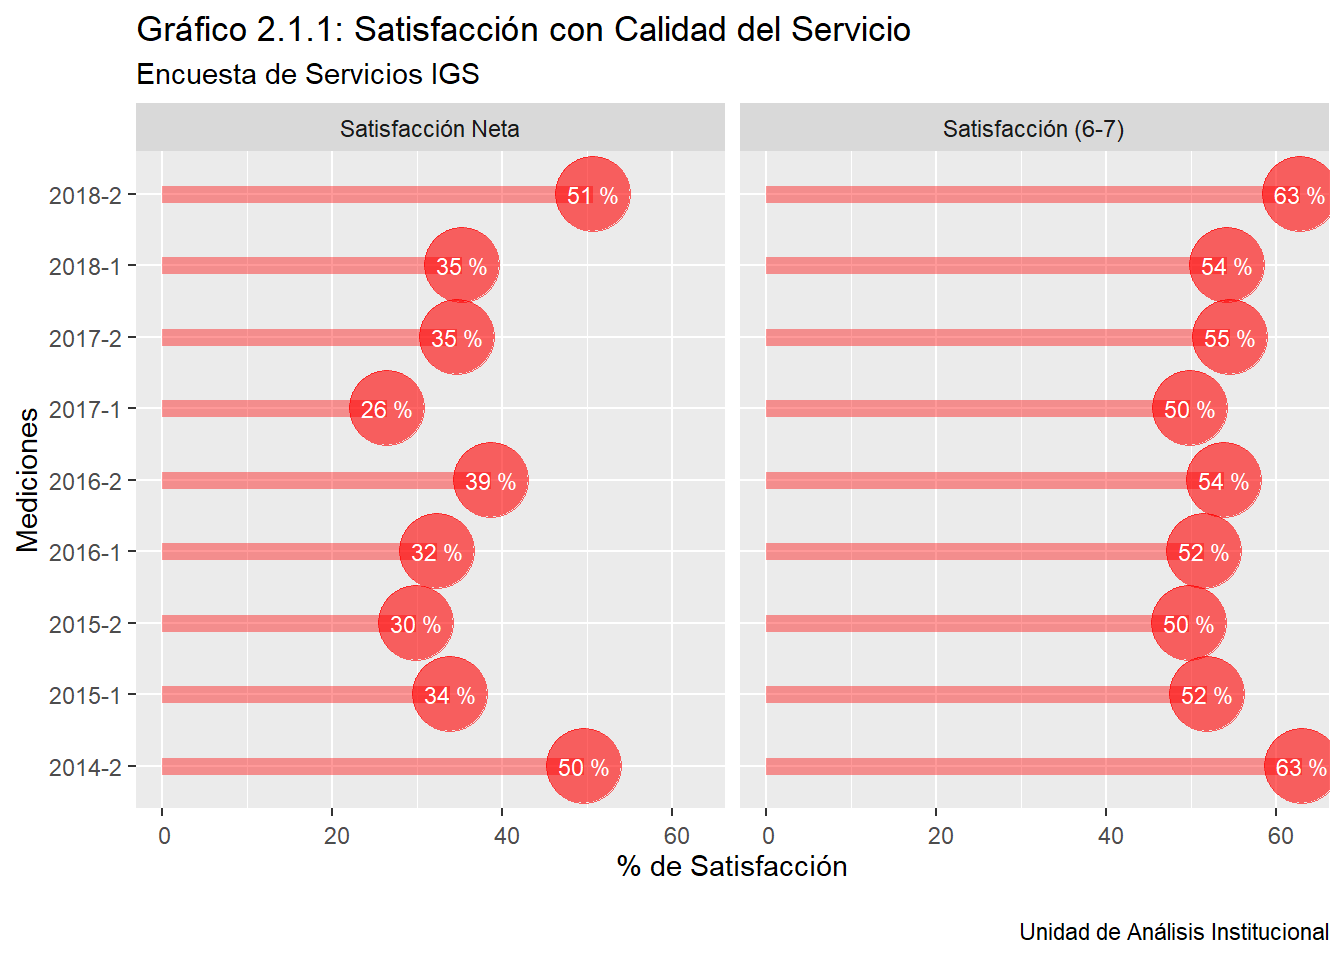
\includegraphics{bookdown_intro_files/figure-latex/unnamed-chunk-5-1.pdf}

En el siguiente gráfico, se evalúa sólo el valor de la
\emph{satisfacción neta} a nivel de cada una de las sedes del Instituto.
Este dato permite apreciar las fluctuaciones que expresa la satisfacción
neta, una fluctuación cuyos valles y peak son más acentuados en la sede
de \textbf{Concepción} y \textbf{Viña del Mar}. Por el contrario, estos
valores fluctúan con menos intensidad y dentro de un espectro de valores
más altos en las sedes de \textbf{Temuco} y \textbf{Rancagua}. Se puede
apreciar que \textbf{Santiago} manifiesta valores históricamente más
bajos, alcanzando en la medición 2018-2 tan sólo 36\%.

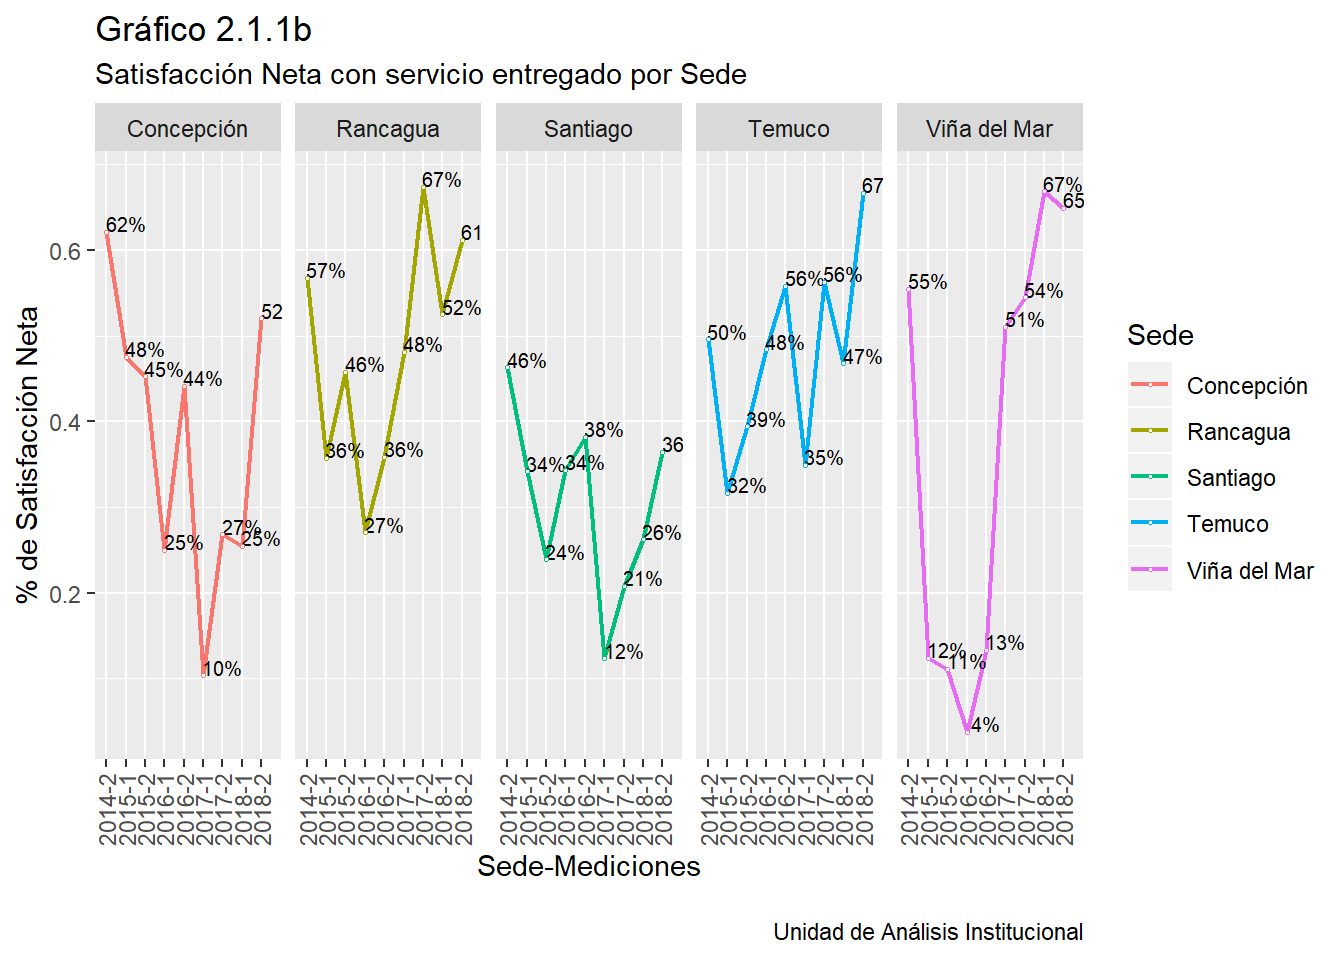
\includegraphics{bookdown_intro_files/figure-latex/unnamed-chunk-7-1.pdf}

** Jornada **

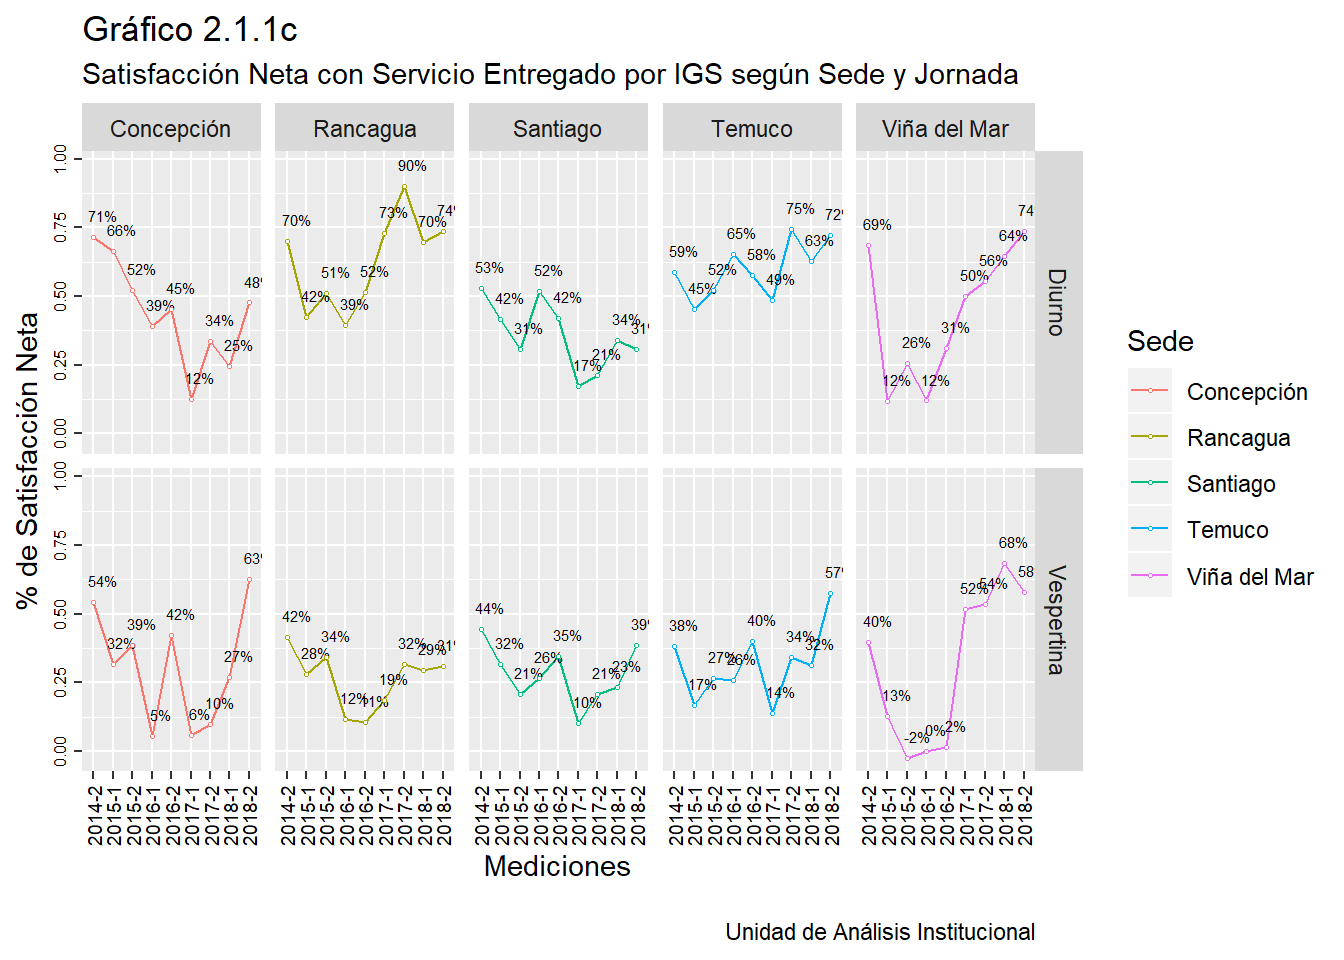
\includegraphics{bookdown_intro_files/figure-latex/unnamed-chunk-9-1.pdf}

\textbf{2.1.2) Percepción de la Calidad de la Atención del IGS}

Otro de los indicadores globales de calidad del servicio, hace
referencia a la \emph{calidad de la atención que recibe el estudiante}.
Esta variable debe ser analizada en mutua complementación con la
variable anterior, puesto que expresa una alta correlación conceptual, y
a su vez, estadística. Esta es una variable ``nueva'', en cuanto que
sólo ha sido medida en las últimas 3 ocasiones (desde 2017-2). Se puede
apreciar, que tal como la variable anterior, esta variable expresa un
alza relevante, específicamente de 22 puntos porcentuales en cuanto a la
\emph{Satisfacción neta} y en más de 13 puntos en cuanto la
\emph{Satisfacción total (6-7)}. Por ende, esta tendencia avala y
consolida lo registrado en la variable revisada en el acápite anterior.

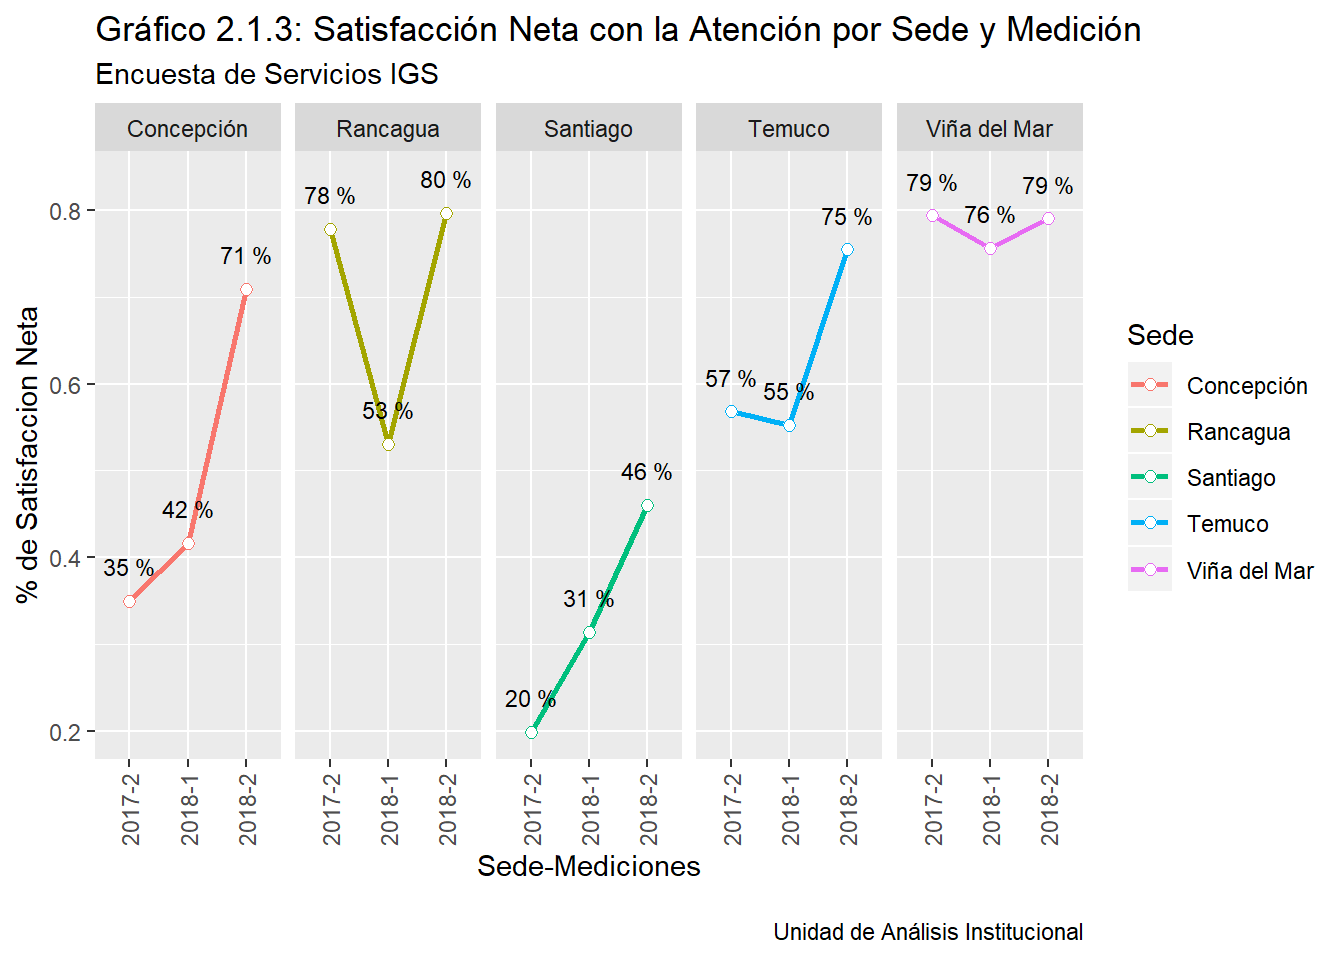
\includegraphics{bookdown_intro_files/figure-latex/unnamed-chunk-10-1.pdf}

Al inspeccionar el comportamiento de la variable por sede, se aprecia un
comportamiento de alza-descenso-alza en las sedes de \emph{Rancagua} y
\emph{Viña del Mar}, aunque en la primera de ellas es más estable en
torno a un rango de valores más altos. Se puede apreciar que las sedes
de \emph{Concepción} y \emph{Temuco} registran un repunte significativo
respecto de la medición anterior; en este mismo aspecto se debe incluir
a \emph{Viña del Mar}. Por último, \emph{Santiago} refleja una tendencia
al alza, aunque sus valores son -en general- más bajos respecto de las
otras sedes.

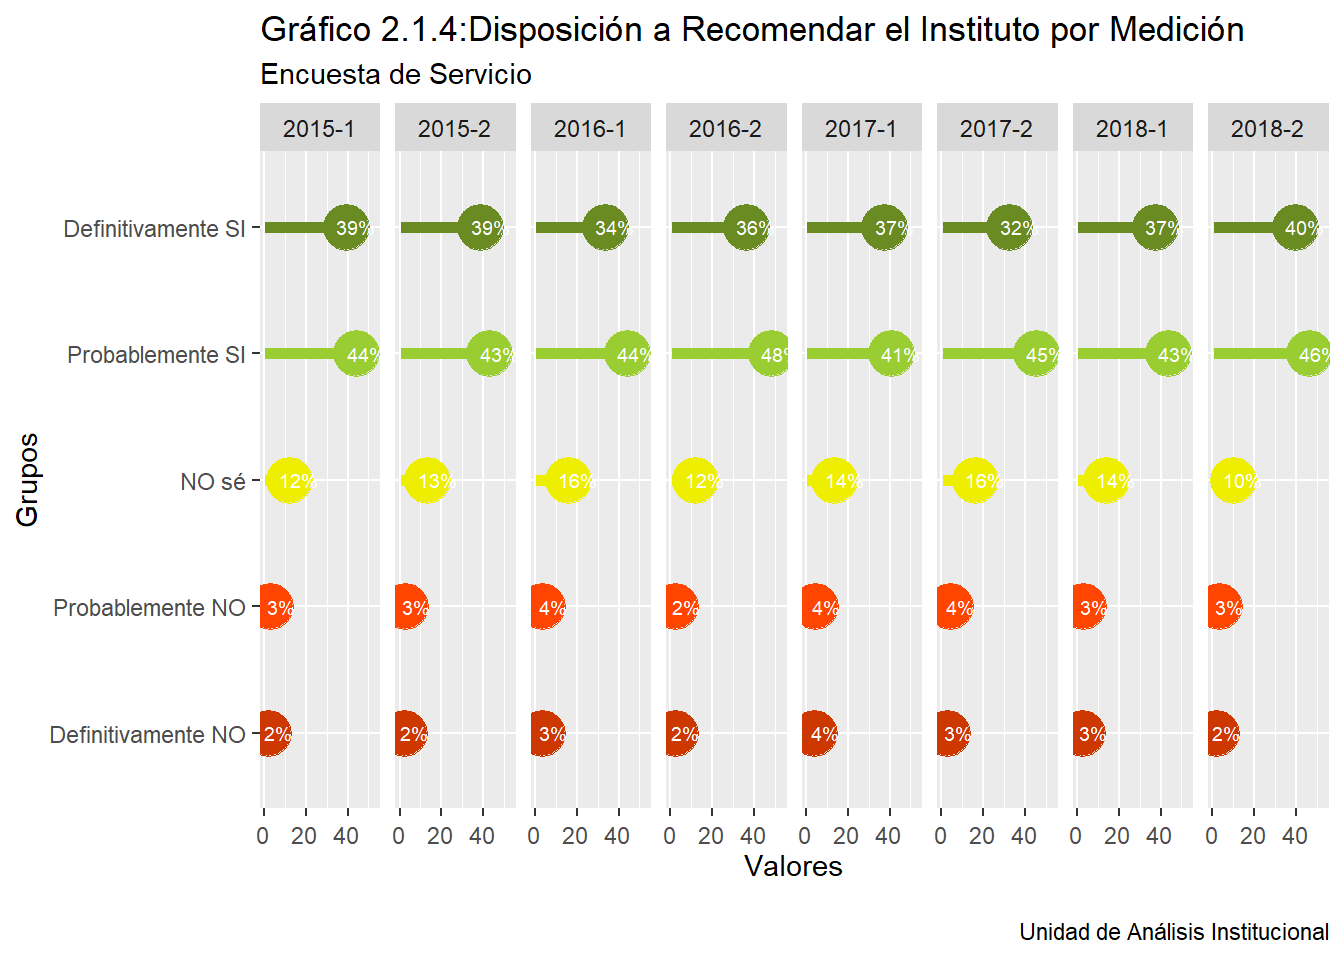
\includegraphics{bookdown_intro_files/figure-latex/unnamed-chunk-12-1.pdf}

\section{Atencion por jornada}\label{atencion-por-jornada}

** Jornada **

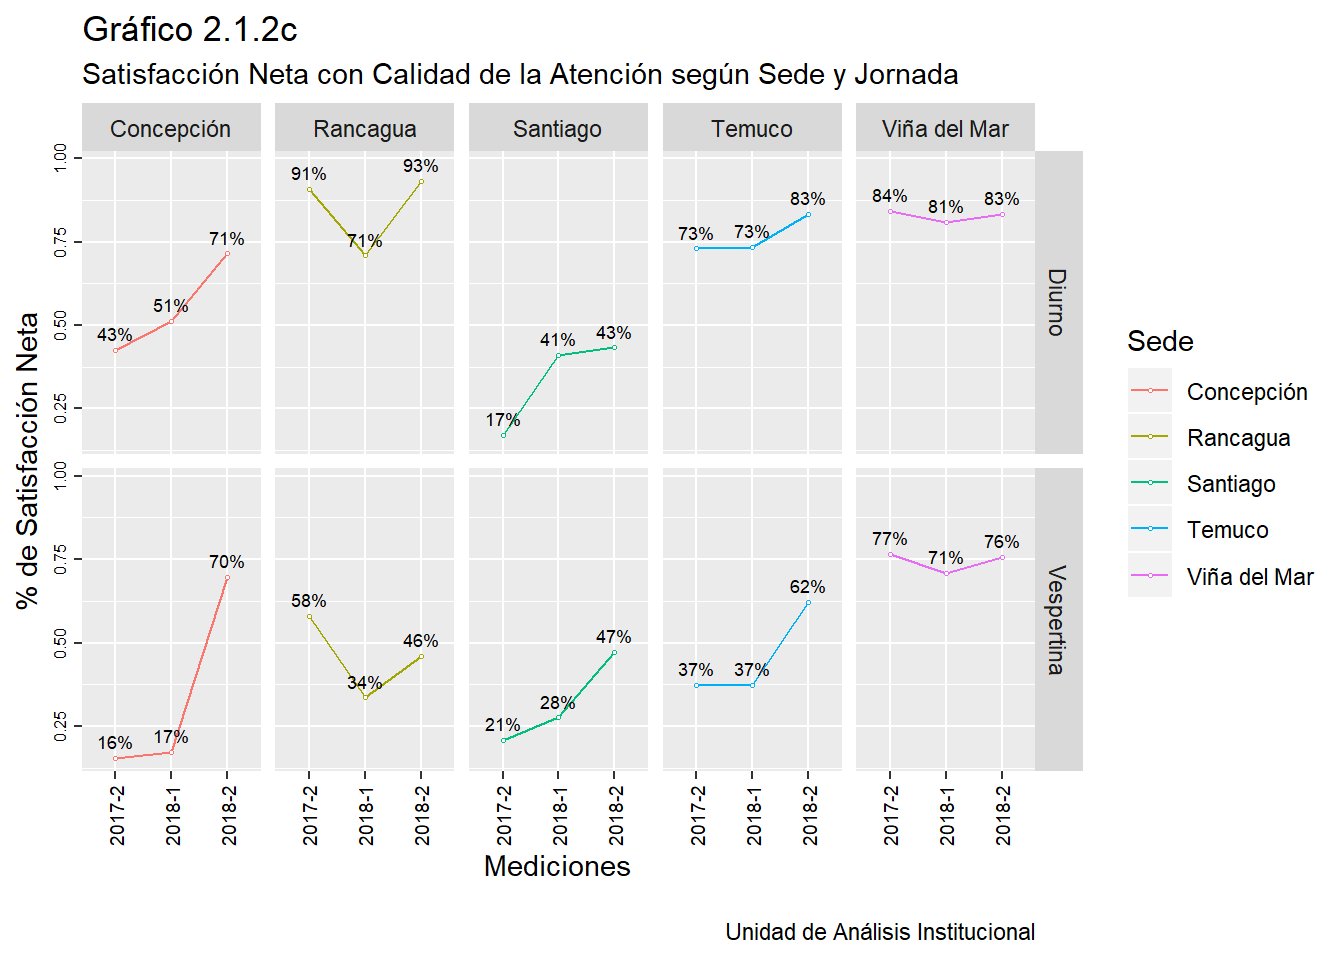
\includegraphics{bookdown_intro_files/figure-latex/unnamed-chunk-14-1.pdf}

\textbf{2.2.3) Disposición a Recomendar el IGS}

La disposición a recomendar un servicio determinado, especialmente si
esta persona es un familiar o amigo(a), expresa en sí mismo una
experiencia positiva del uso de dicho servicio. Al observar las cifras
en este ámbito, se aprecia que la disposición a recomendar el Instituto
Subercaseaux alcanza un 86\%, sumando aquellos estudiantes que dicen que
con toda claridad lo harían (``Definitivamente: 40\%''), junto con
aquellos que lo indican como una probabilidad cierta
(``Probablemente:46\%''). Esta cifra expresa un alza de 6 puntos
respecto del dato registrado en la medición anterior (2018-1).

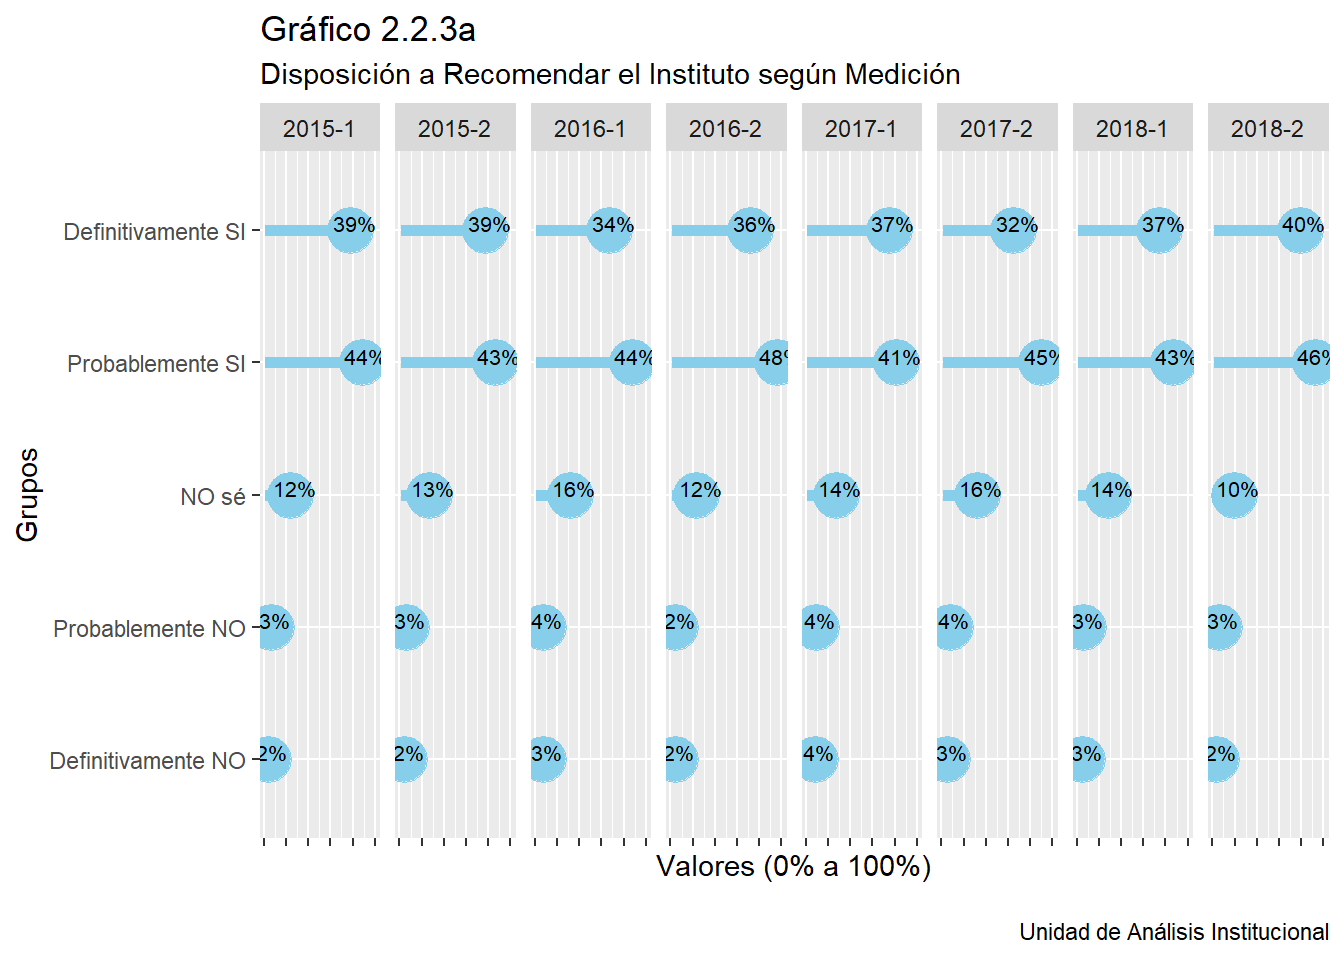
\includegraphics{bookdown_intro_files/figure-latex/unnamed-chunk-16-1.pdf}

El gráfico siguiente muestra el porcentaje de estudiantes que tienen una
disposición positiva frente a la posibilidad de recomendar el Instituto.
Los valores en este dato son más altos, tanto en la actual medición como
en las anteriores; esta tendencia se repite en cada una de las sedes. En
este sentido, se constata un desacoplamiento del dato respecto de las
últimas dos variables generales revisadas anteriormente. Al parecer, el
dato y su tendencia expresan una satisfacción \emph{de base} donde
convergen otros elementos y aspectos conectados con la trayectoria de
los estudiantes.

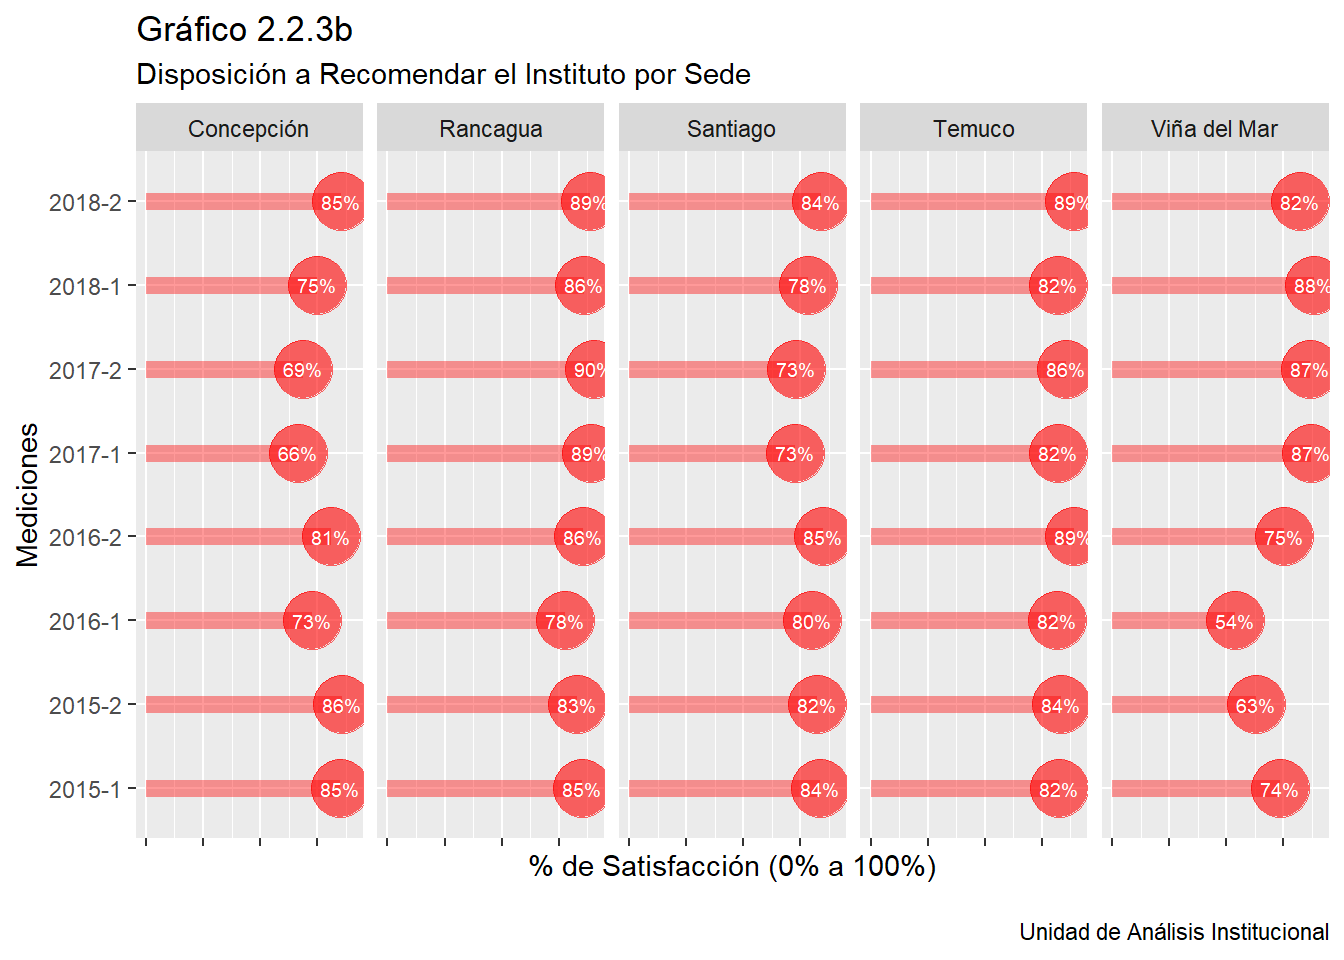
\includegraphics{bookdown_intro_files/figure-latex/unnamed-chunk-18-1.pdf}

\section{Satisfacción con Docentes}\label{satisfaccion-con-docentes}

Dentro de los actores del Instituto, los docentes ocupan un puesto
estratégico dado que son ellos/as quienes interactúan de forma cotidiana
con los estudiantes, una interacción que es fruto de la función
pedagógica propia del Instituto. En este sentido, sus desempeños -en
términos amplio- es parte de ese conjunto de elementos intangible que
los estudiantes tienen presente al momento de generar una opinión. En el
siguiente gráfico, se aprecia la satisfacción neta y total,
registrándose en ambas un incremento de 9 y de 6 puntos,
respectivamente.

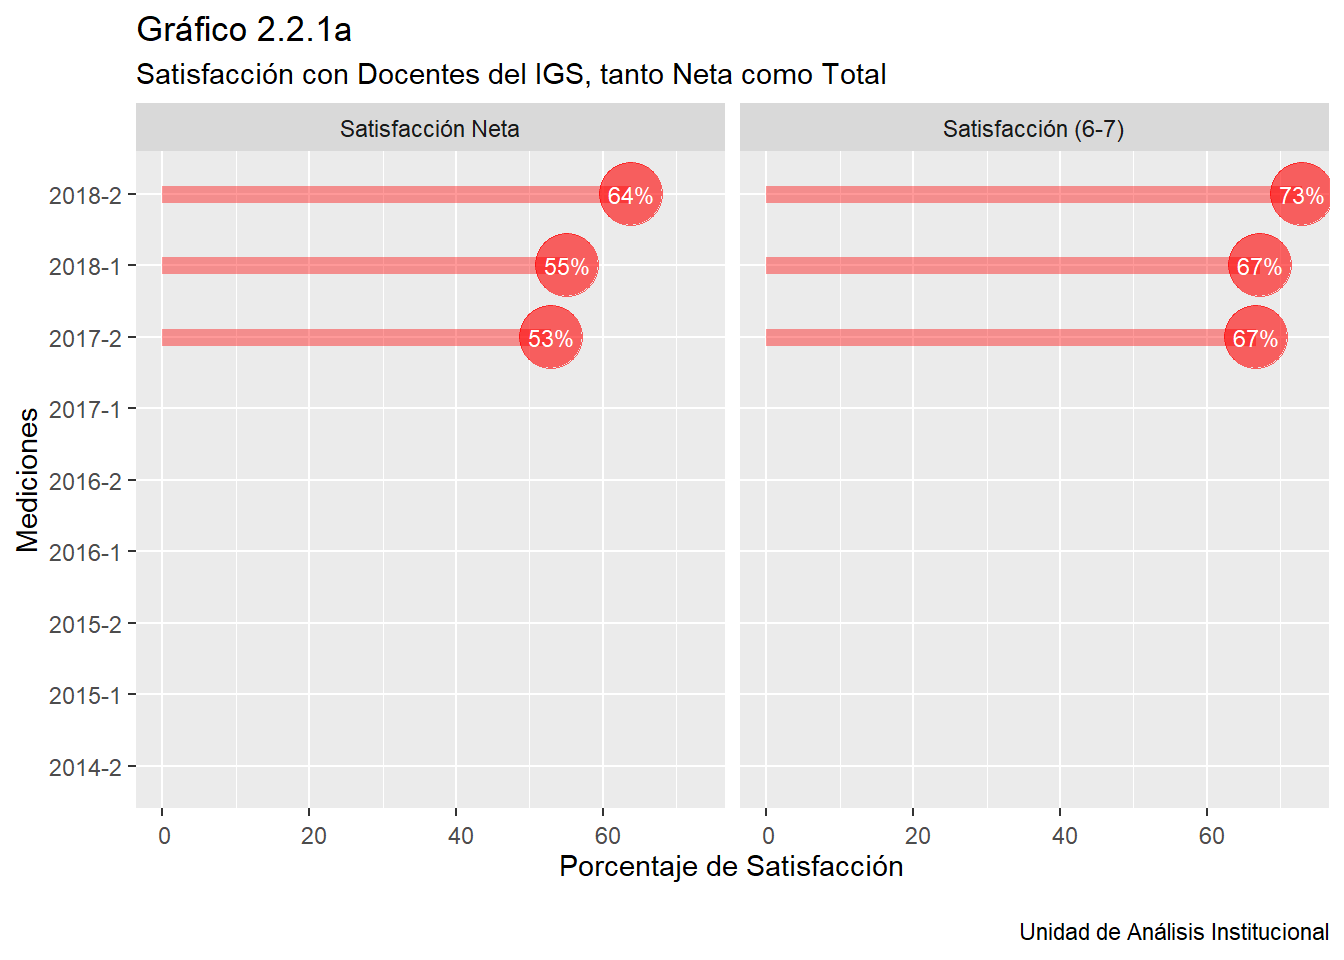
\includegraphics{bookdown_intro_files/figure-latex/unnamed-chunk-19-1.pdf}

A nivel de cada una de las sedes, la satisfacción neta de los
estudiantes con los docentes muestra diferencias relevantes. La
satisfacción neta es más alta (en las últimas 3 mediciones), en las
sedes de \emph{Rancagua} y \emph{Temuco}; esto más allá de que en ambas
se registre un descenso en la medición 2018-1. La sede de
\emph{Concepción} tiene un descenso en la medición de 2018-1, pero se
recupera en la medición (2018-2). La sede de \emph{Viña del Mar} es
bastante estable en las tres mediciones, en torno al 68\% de
satisfacción neta. Por último, en la sede de \emph{Santiago} la
satisfacción neta es baja, y aunque ha venido al alza, aún no supera el
umbral del 50\%.

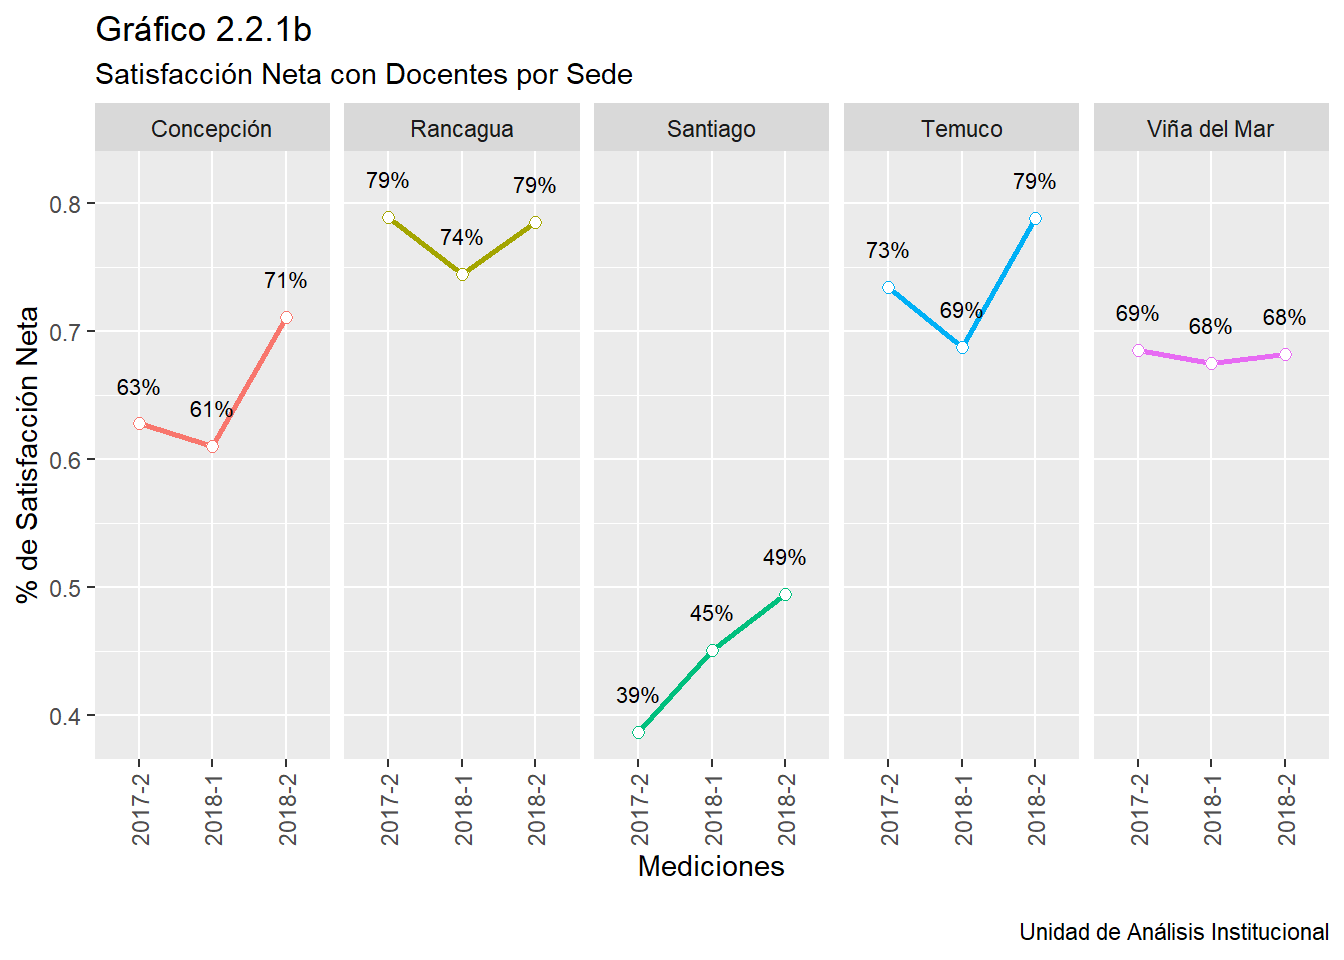
\includegraphics{bookdown_intro_files/figure-latex/unnamed-chunk-21-1.pdf}

** Jornada **

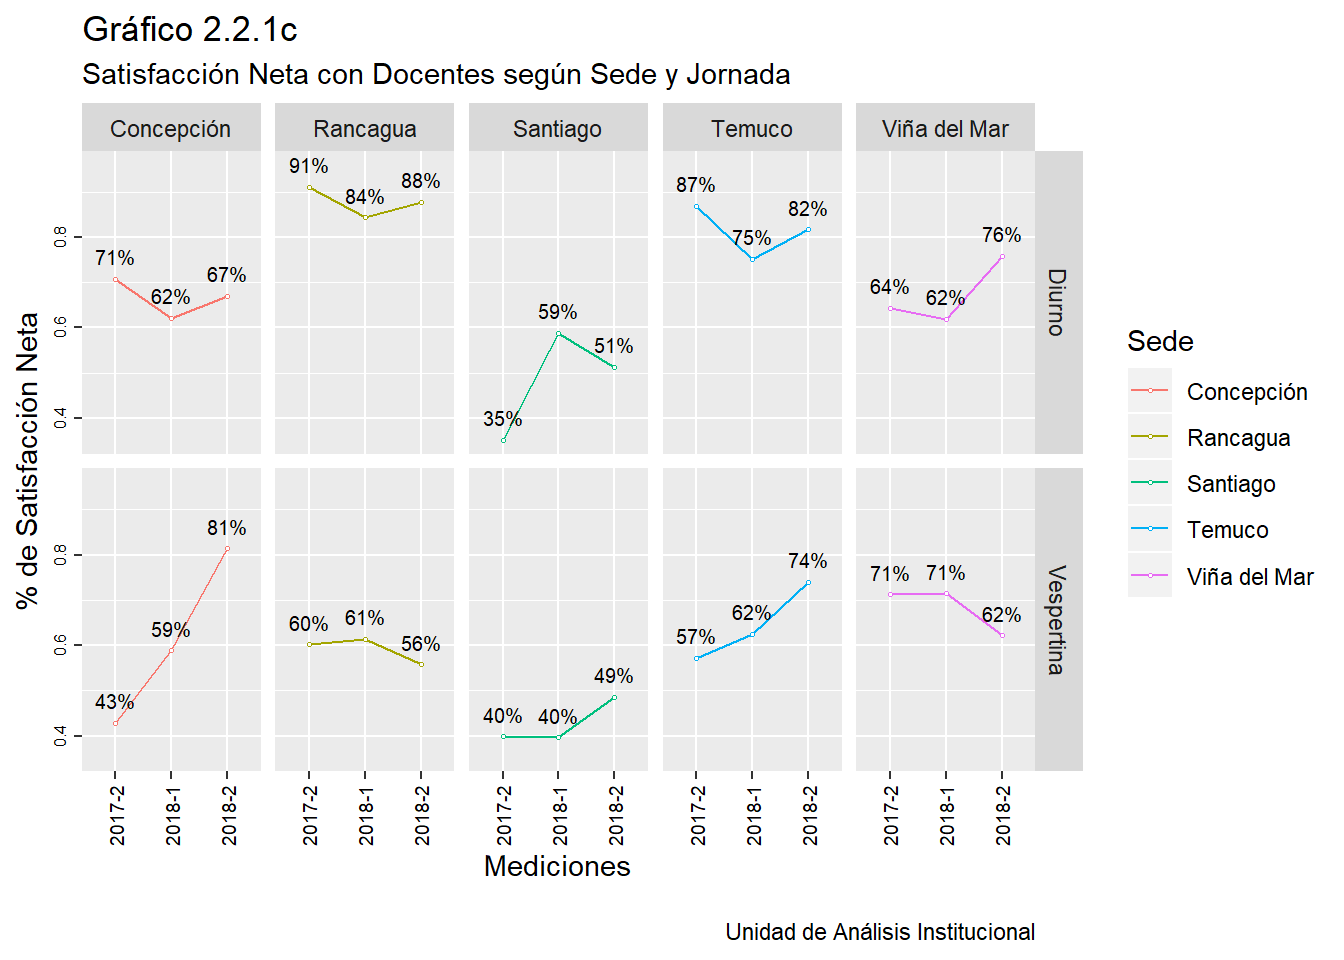
\includegraphics{bookdown_intro_files/figure-latex/unnamed-chunk-23-1.pdf}

En este ámbito, dentro del cuestionario se consulta a aquellos
estudiantes que evalúan con una nota inferior a 7 a los docentes, sobre
cuáles -desde su perspectiva- son las mejoras (cambios) que debiesen
suceder para lograr un óptimo de satisfacción con el desempeño docente.
En el siguiente gráfico, se ha desglosado el dato por cada sede para
acercarnos a fenómenos más localizados. Es posible apreciar que en cada
una de las sedes lo que se sugiere es mejorar la \emph{``metodología''}
de enseñanza, junto con ello aparece como sugerencia el hecho de mejorar
la \emph{``comunicación o claridad expositiva en clases''}.

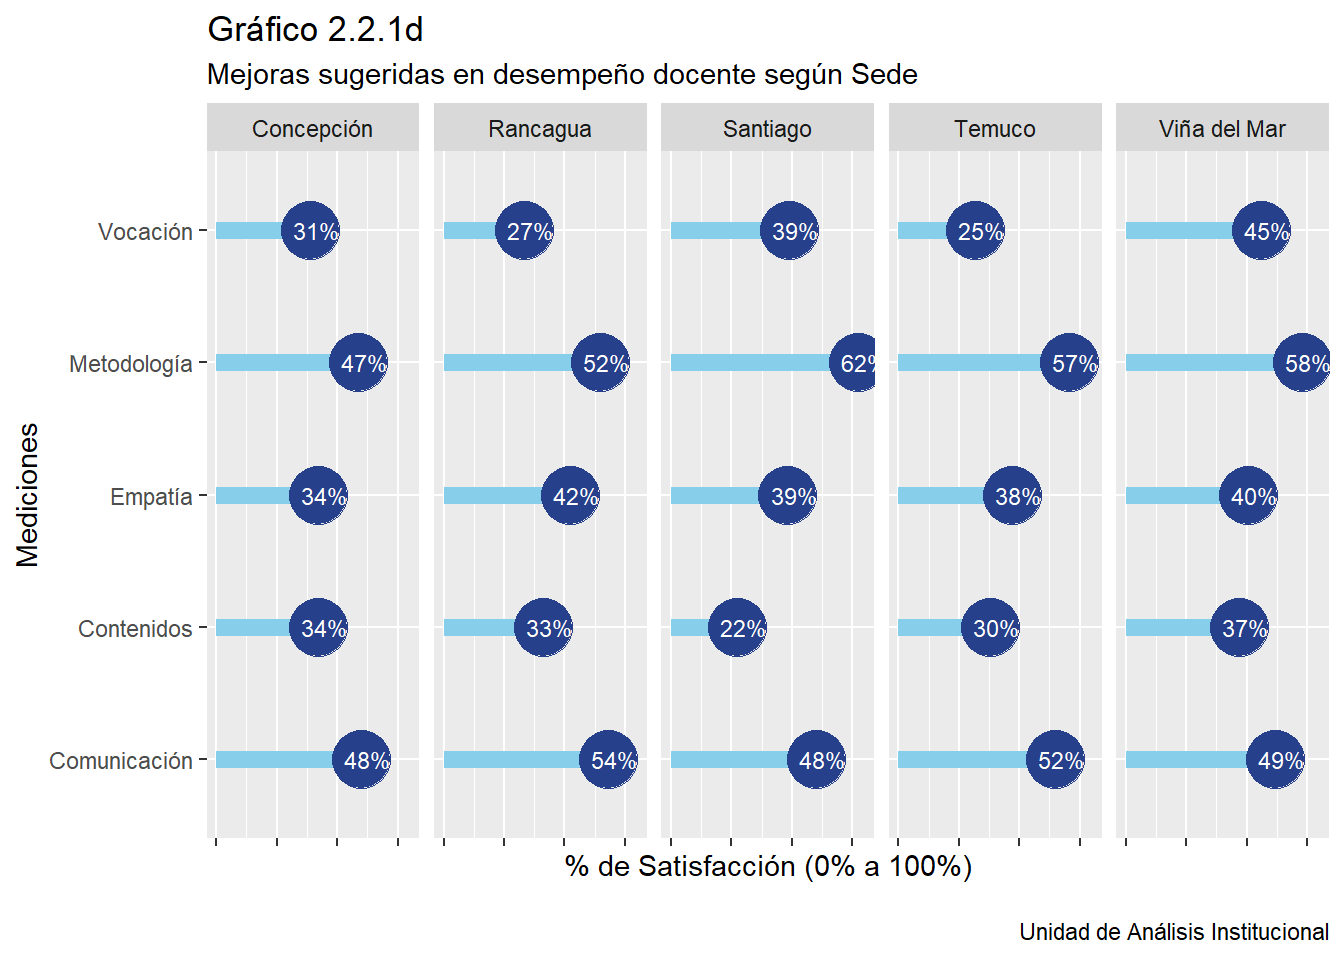
\includegraphics{bookdown_intro_files/figure-latex/unnamed-chunk-25-1.pdf}

\section{Satisfacción con la Infraestructura y Otros Espacios Físicos
del
IGS}\label{satisfaccion-con-la-infraestructura-y-otros-espacios-fisicos-del-igs}

\textbf{2.3.1. Satisfacción con la Infraestructura}

En el siguiente gráfico, se aprecia la satisfacción neta y total en las
últimas 3 mediciones. Se aprecia que ha existido un alza sistemática,
aunque leve. Los valores indican que la satisfacción neta está en torno
al 50\% y la satisfacción total en torno al 65\%.

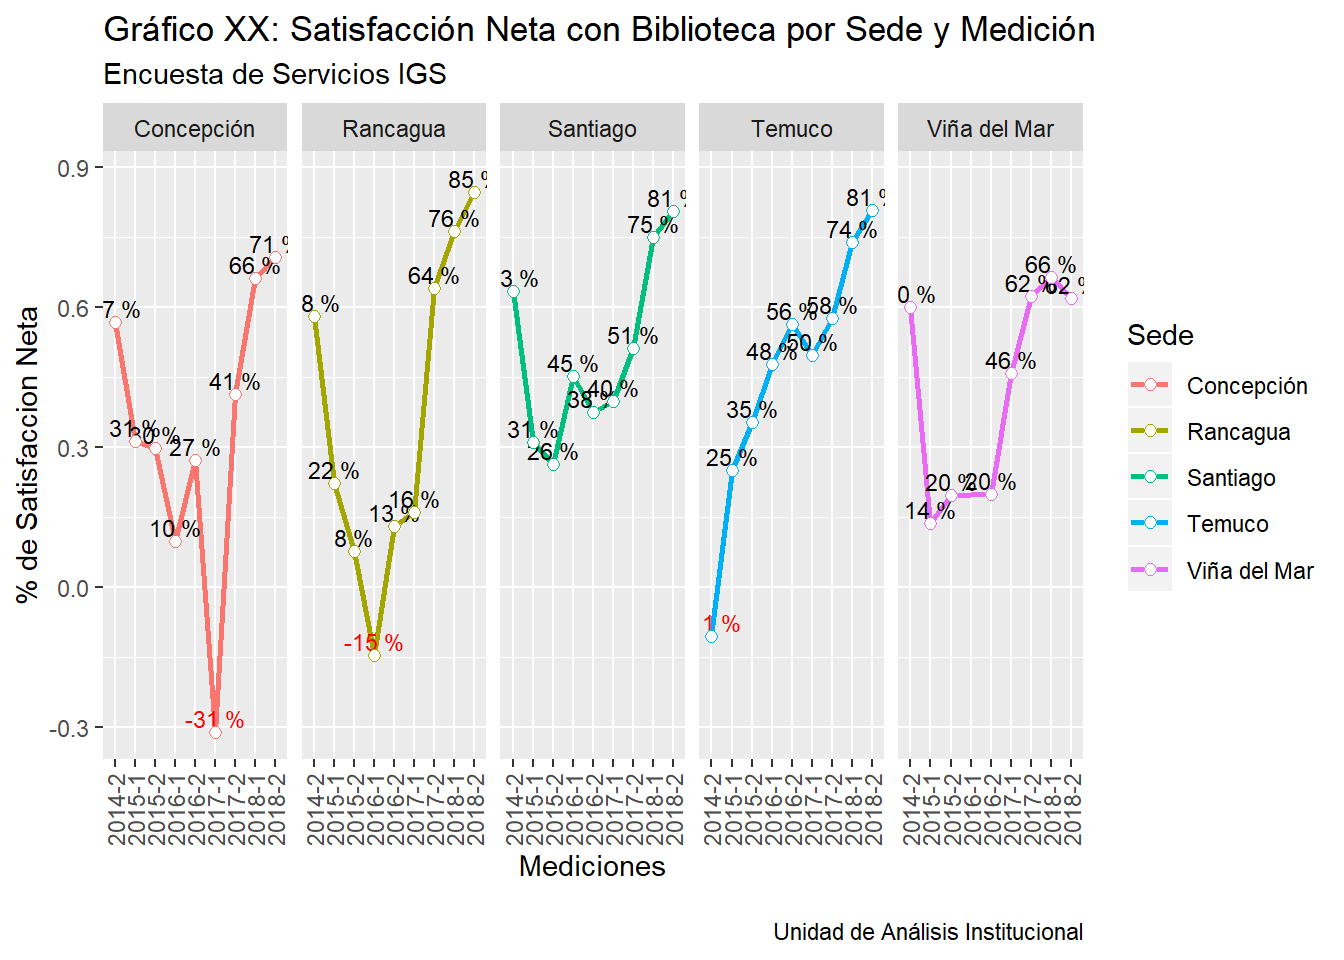
\includegraphics{bookdown_intro_files/figure-latex/unnamed-chunk-26-1.pdf}

El siguiente gráfico permite analizar la satisfacción con la
infraestructura, pero a su vez aquellos espacios que especifican de
mejor forma, aunque no completamente, su ámbito. Revisando el gráfico
siguiente, es posible apreciar que el espacio de
\emph{Cafetería/Casino}, corresponde a aquél que genera un menor grado
de satisfacción neta. Por otro lado, ya desde 2017-2, el espacio de
\emph{Biblioteca} registra un alza en la satisfacción neta que alcanza
en la medición actual un 78\%. Otro servicio que ha tenido un repunte
consistente corresponde a \emph{Baños}, alcanzando un 61\% en la última
medición. Partiendo de un piso algo más alto, el espacio de \emph{salas
de clases} también registra un alza sostenida. Por último, laboratorios
es el espacio que manifiesta mayor estabilidad en las diferentes
mediciones.

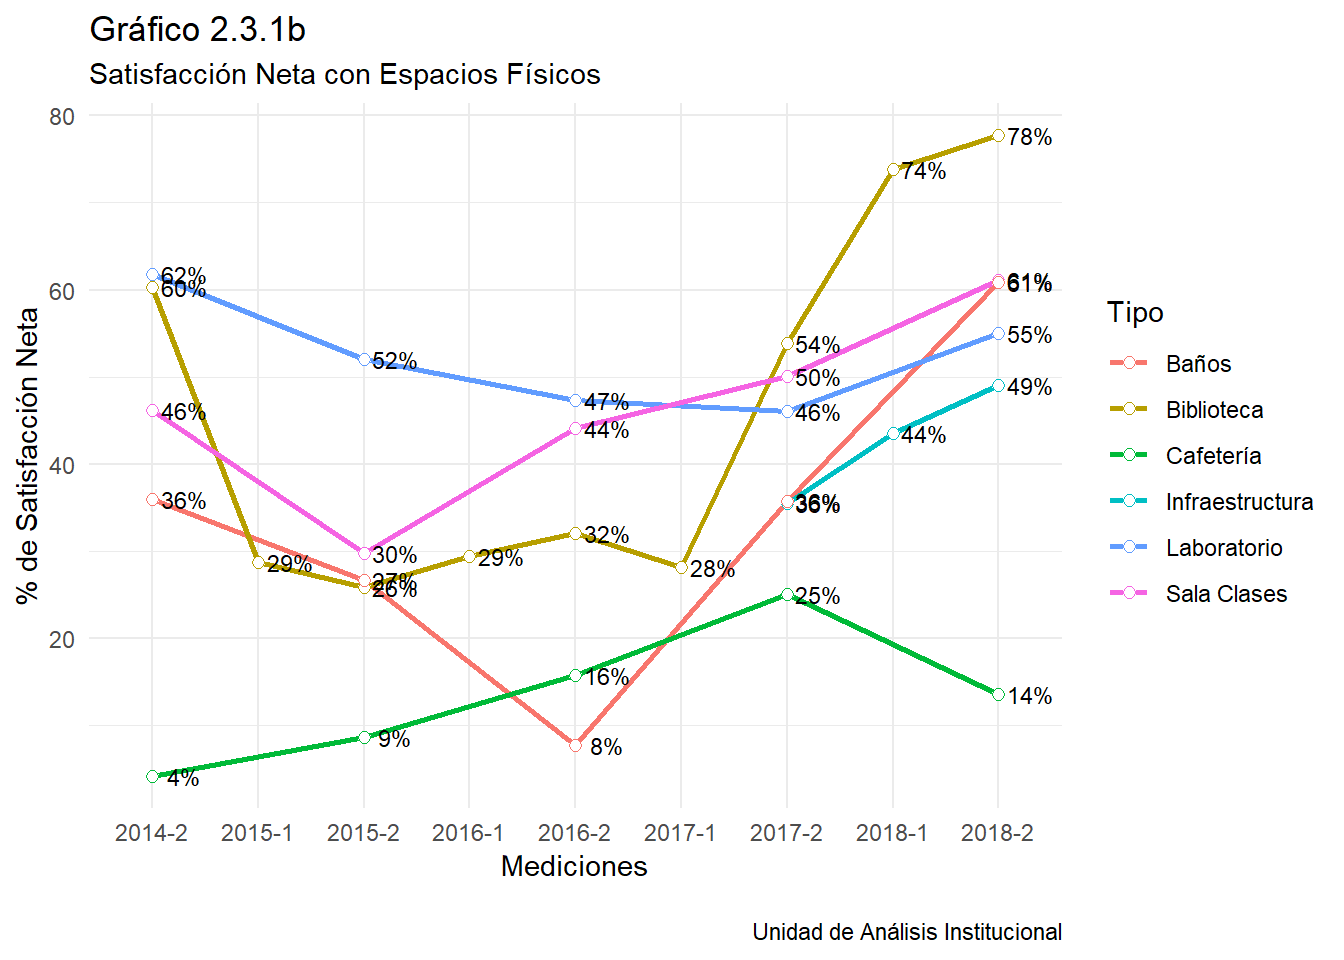
\includegraphics{bookdown_intro_files/figure-latex/unnamed-chunk-28-1.pdf}

La satisfacción con la infraestructura a nivel de cada sede se plasma en
el siguiente gráfico. Es posible apreciar que \emph{Rancagua} registró
en la medición 2017-2 el valor más alto de satisfacción neta, aunque
después descendió en torno al 60\%. Se les asimila la dinámica que
muestran las sedes de \emph{Temuco} y \emph{Viña del Mar}. La sede de
\emph{Santiago} registra una satisfacción neta históricamente baja, no
superando el 50\%. No obstante, aún más bajo es la satisfacción en la
sede de \emph{Concepción}, donde el valor es incluso negativo (-16\%).
Además, en esta última sede, el valor más alto se registró en 2017-2,
pero sólo alcanzó 11\%, luego bajo al 7\% y llegó -en esta última
medición- a la cifra antes indicada.

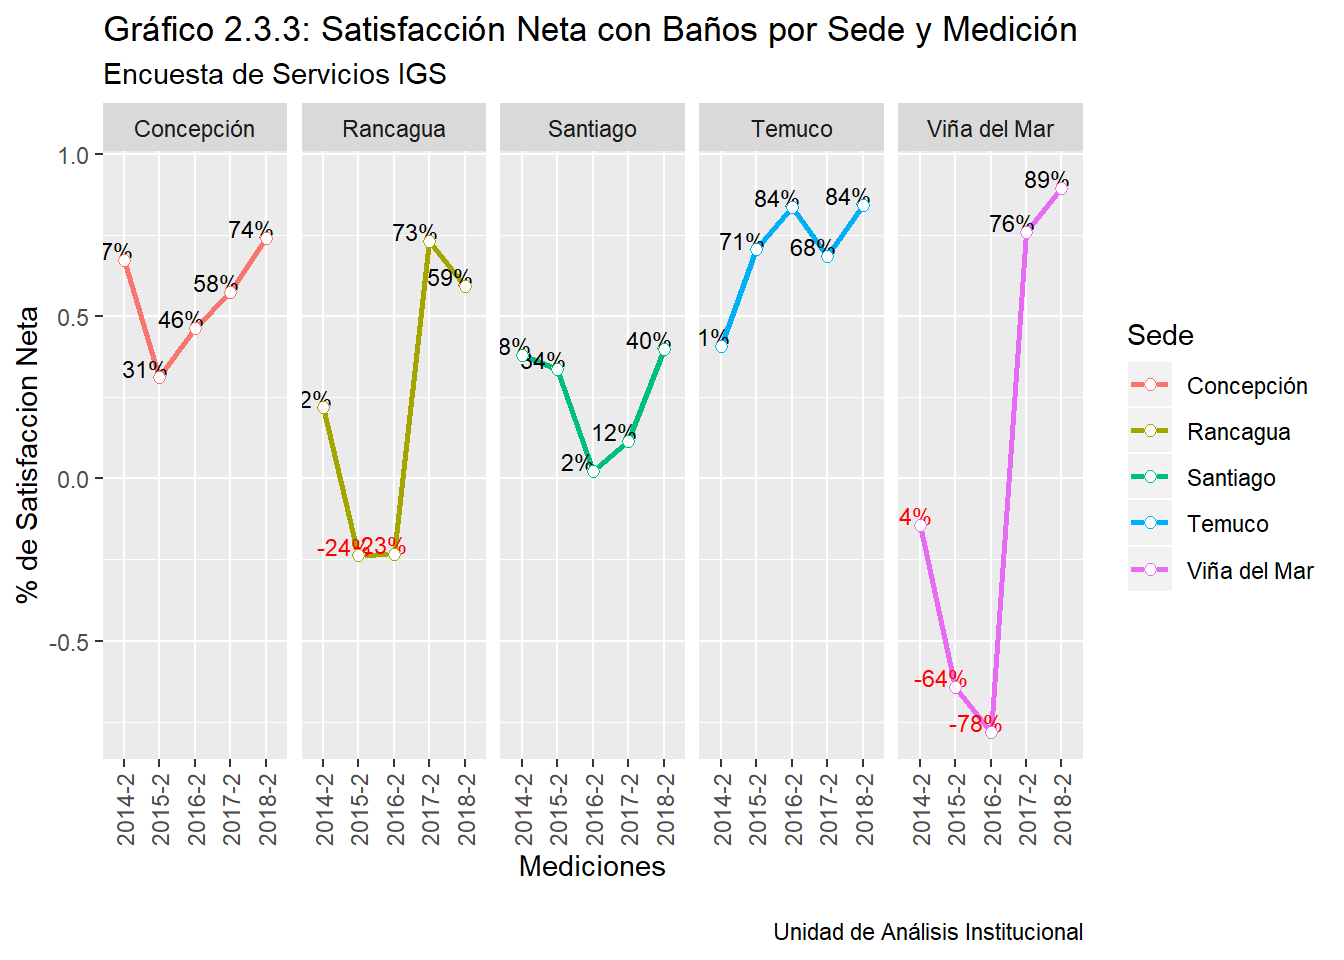
\includegraphics{bookdown_intro_files/figure-latex/unnamed-chunk-30-1.pdf}

Se les preguntó a aquellos estudiantes que evaluaron con una nota
inferior a 7 la infraestructura de la sede, \emph{¿qué mejoras debiesen
ocurrir para lograr un óptimo de satisfacción en este ámbito?}. En
infraestructura, lo que se sugiere es diferente según la realidad de
cada sede. Por ejemplo, en \emph{Rancagua} y \emph{Viña del Mar} se
solicita de forma clara mejorar la \textbf{Cafetería}. En tanto en
\emph{Concepción} y \emph{Temuco} hay una petición clara por mejorar los
\textbf{Espacios comunes}.

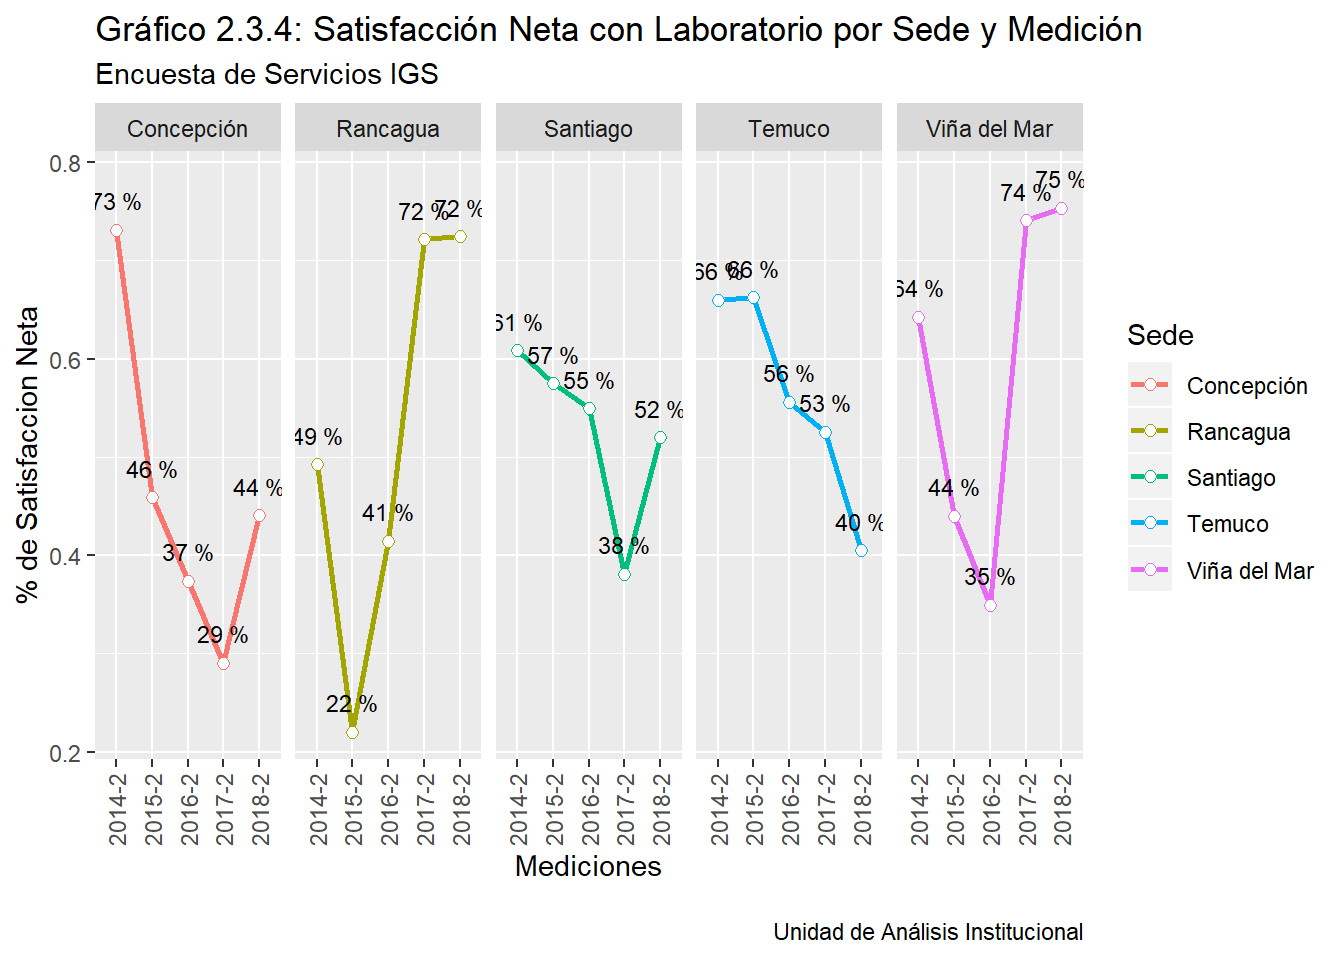
\includegraphics{bookdown_intro_files/figure-latex/unnamed-chunk-32-1.pdf}

** 2.3.2. Salas de Clases**

La satisfacción neta relacionada con la \emph{Sala de Clases} registra
en 2018-2 un 61\%, 11 puntos más respecto de la medición anterior
(2017-2). Al observar cómo se comporta este valor por sede, la tendencia
indica que la satisfacción neta en este ámbito ha aumentado desde una
caída importante en el año 2015, estabilizándose en tres sedes
(\emph{Rancagua}, \emph{Temuco} y \emph{Viña del Mar}). En el caso de
esta última, llegó a registrar valores negativos en los años 2015 y
2016, mejorando de forma significativa los últimos dos años. Por otra
parte, tanto \emph{Concepción} como \emph{Santiago}, registran valores
comparativamente más bajos en este ámbito.

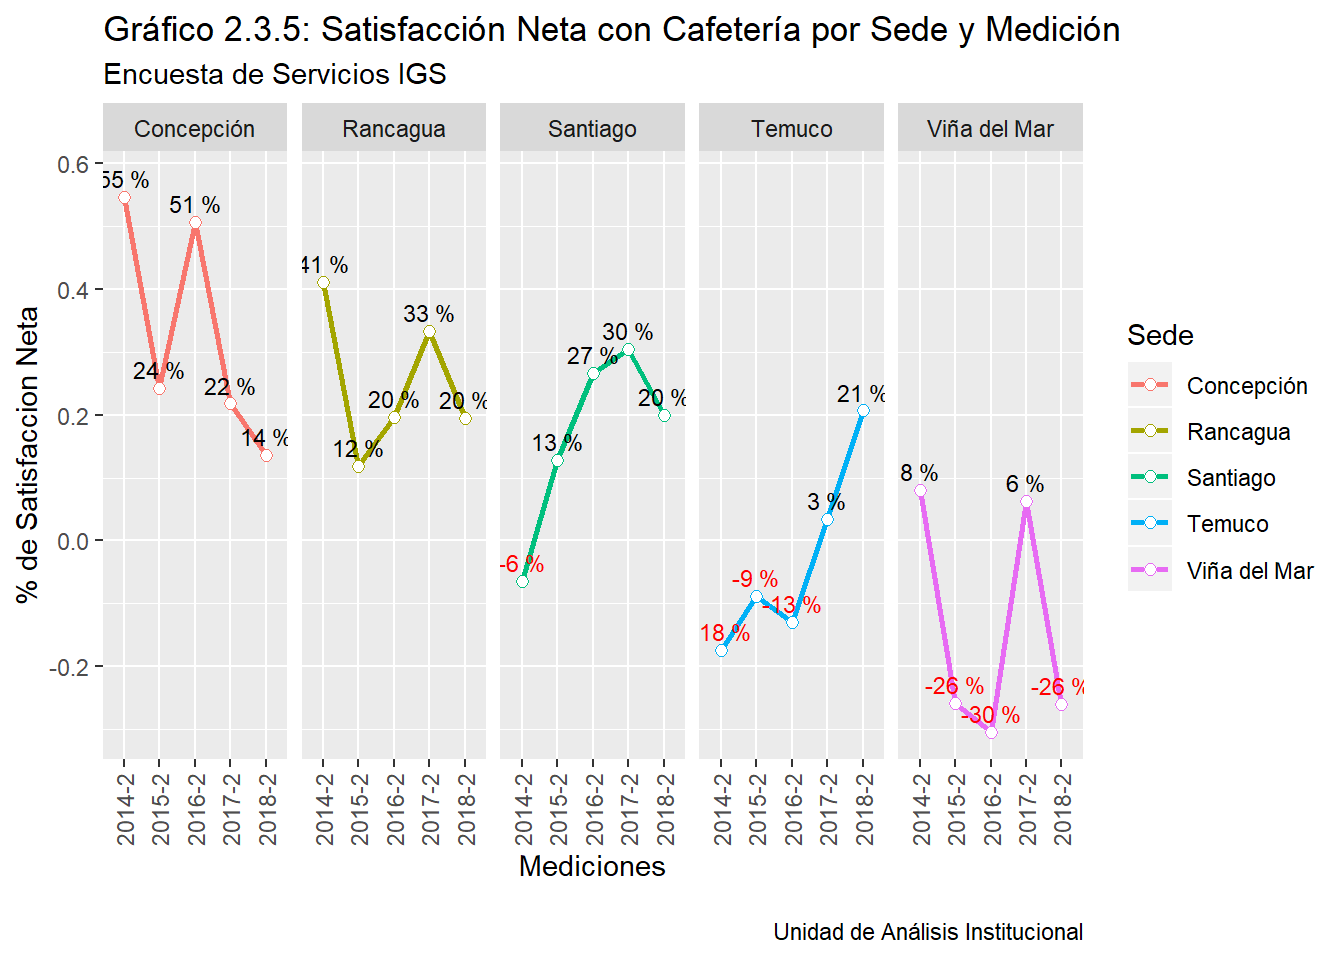
\includegraphics{bookdown_intro_files/figure-latex/unnamed-chunk-34-1.pdf}

** Jornada **

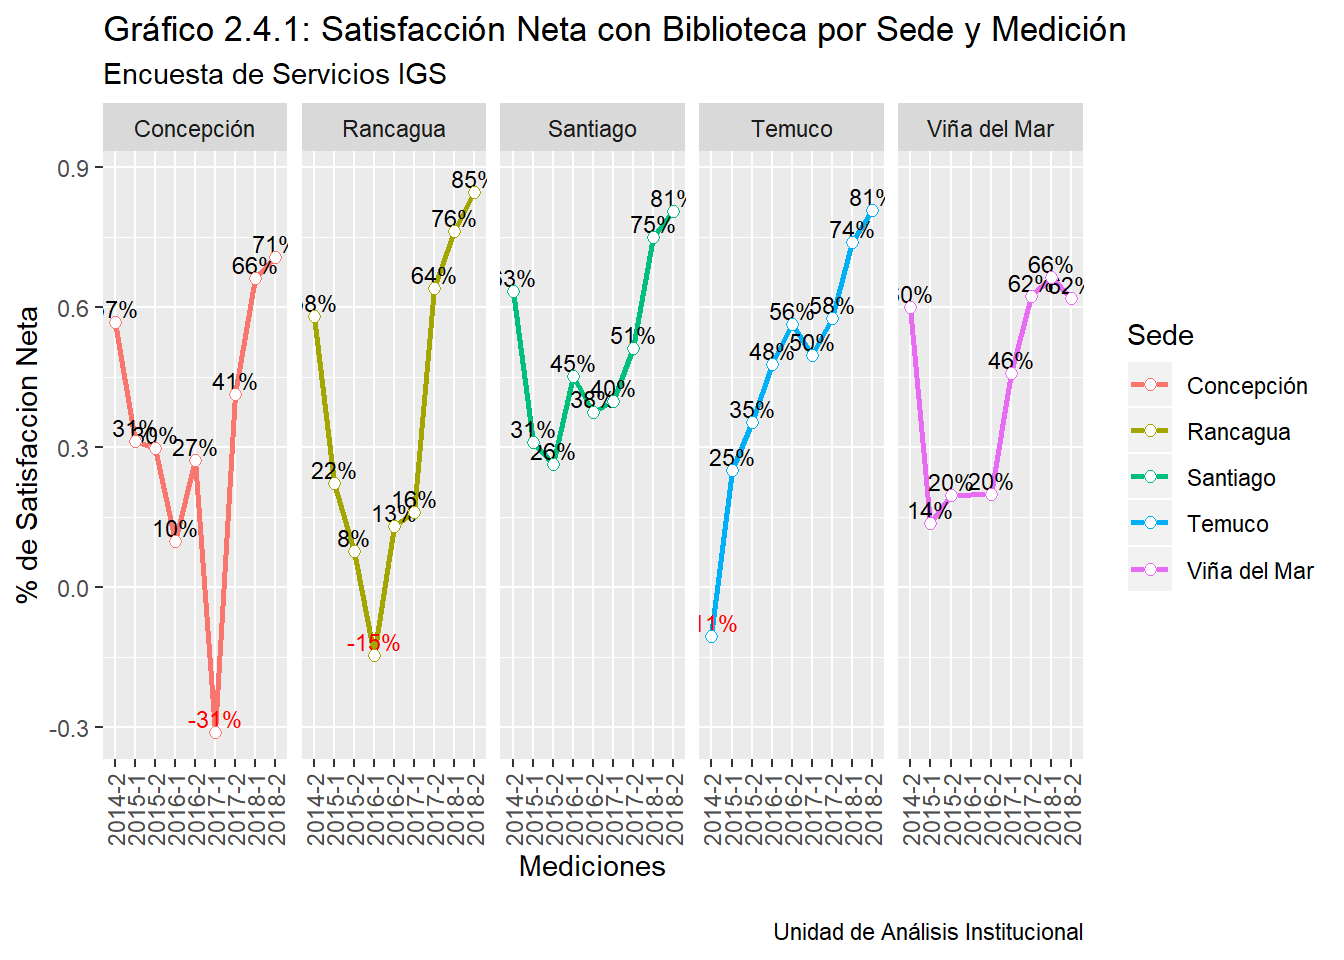
\includegraphics{bookdown_intro_files/figure-latex/unnamed-chunk-36-1.pdf}

** 2.3.3. Baños**

Según se señaló en el acápite referido a infraestructura-Baños, en
2018-2 se registra un 61\% de satisfacción neta, casi el doble del valor
registrado en 2017-2 (36\%). En las sedes \emph{Viña del Mar} y
\emph{Rancagua} se registraron caídas significativas en los años 2015 y
2016. Lo mismo ocurre en las otras sedes, pero de forma menos acentuada.
Todas las sedes, desde que experimentan una caída tienen un alza más o
menos acentuada, aunque sí constante. En este ámbito, es \emph{Temuco}
la sede con mejor desempeño a nivel histórico y \emph{Santiago} aquella
con los valores más bajos.

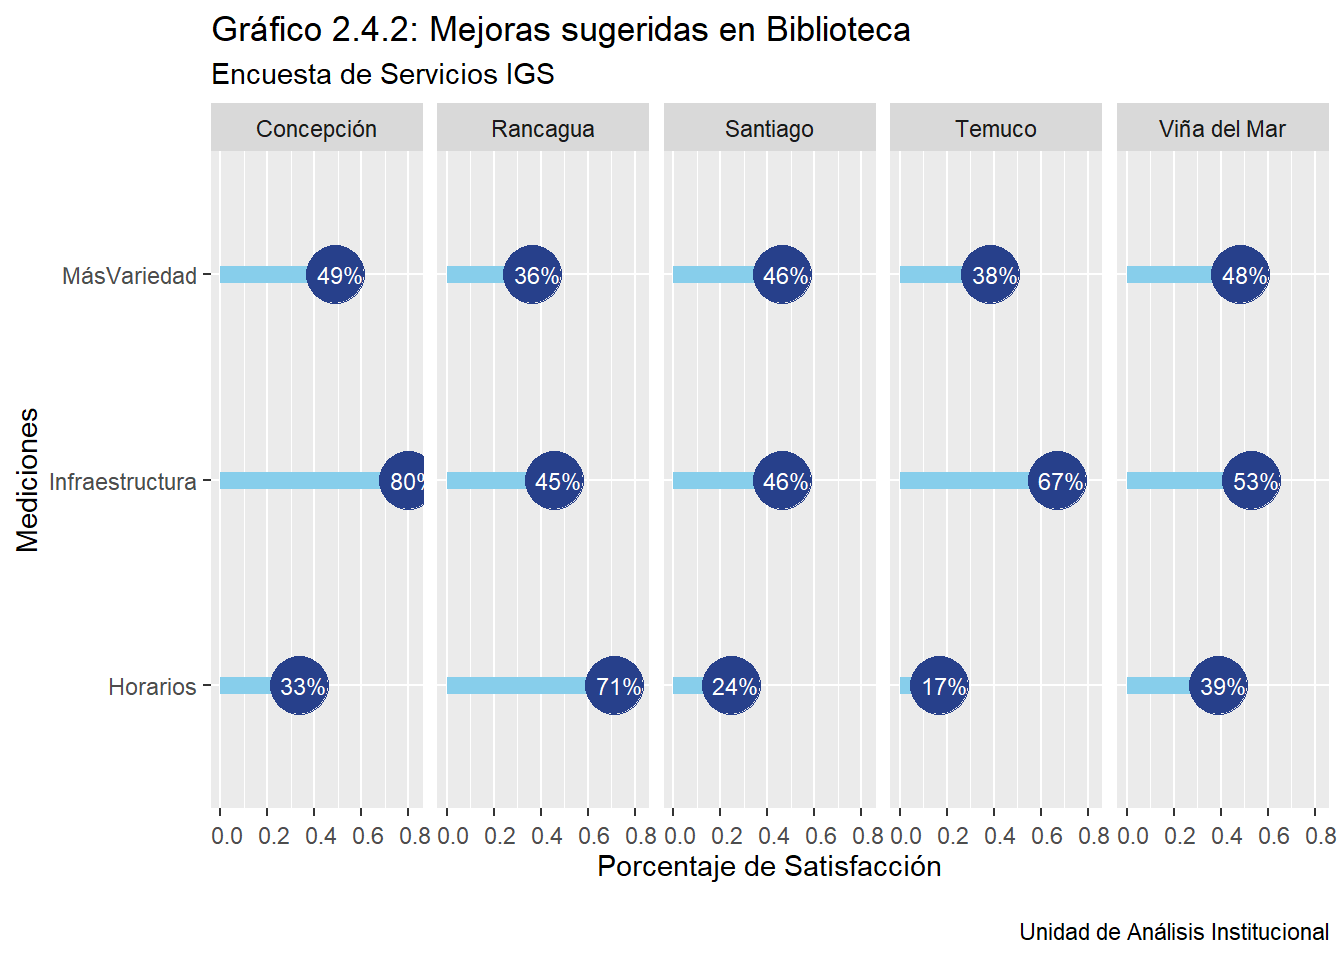
\includegraphics{bookdown_intro_files/figure-latex/unnamed-chunk-38-1.pdf}

** Jornada **

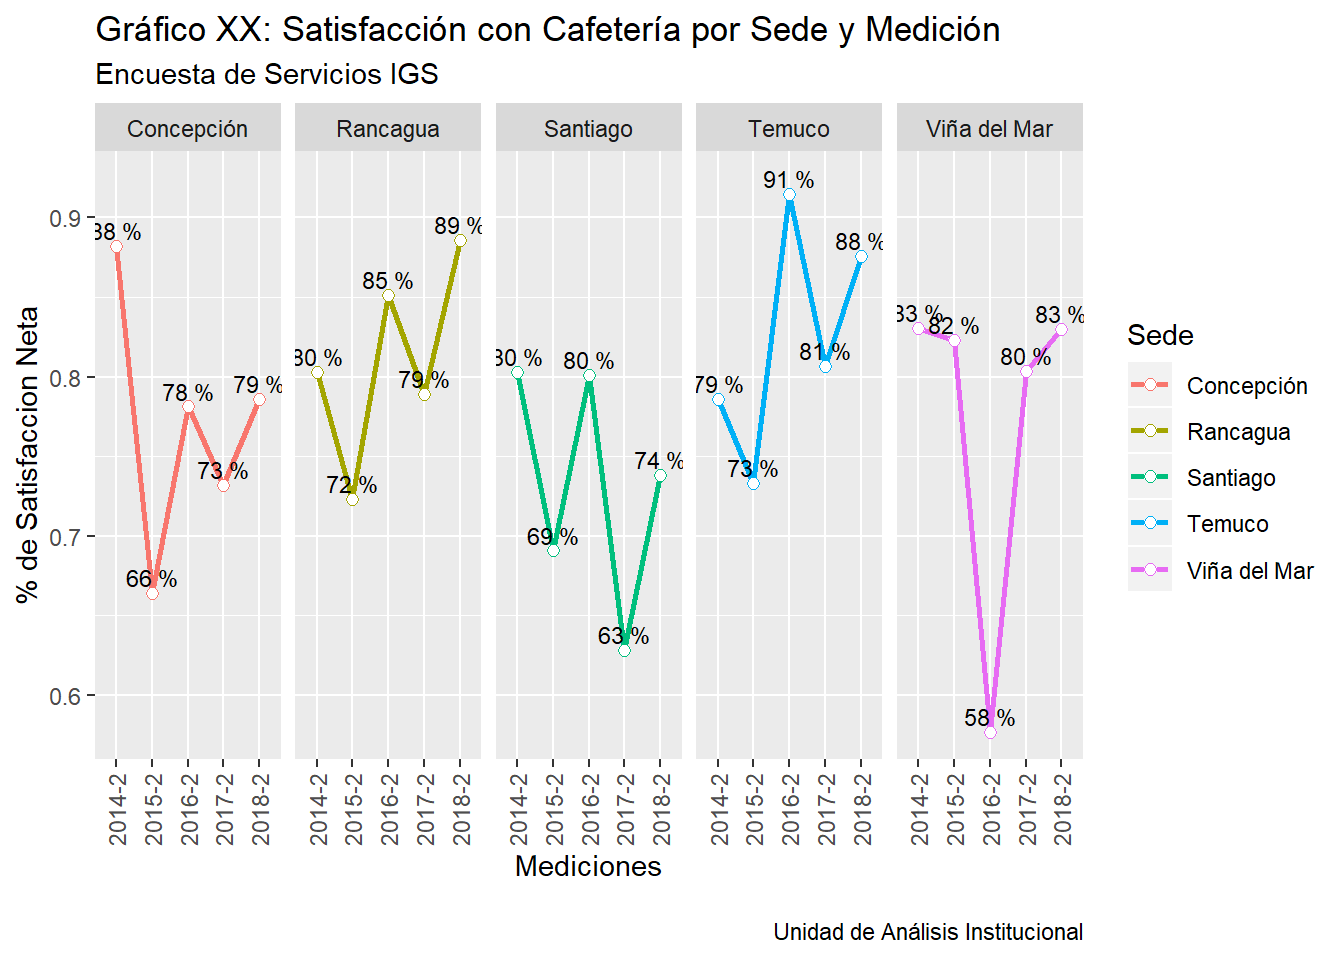
\includegraphics{bookdown_intro_files/figure-latex/unnamed-chunk-40-1.pdf}

** 2.3.4. Laboratorios**

En relación con los laboratorios, se aprecia tendencias a la baja hasta
el año 2017-2 en los casos de \emph{Concepción} y \emph{Santiago},
después de dicho año existe un repunte en la medición actual (2018-2).
En el caso de la primera sede este repunte alcanza al 44\%, en cuanto a
la segunda sede, llega al 52\%. En el caso de \emph{Rancagua} y
\emph{Viña del Mar}, estas caídas ocurren en los años 2015-2 y 2016-2,
respectivamente. No obstante, ambas sedes hoy (2018-2) alcanzan valores
de satisfacción neta en torno al 73\%. Es muy relevante poner atención
al descenso sistemático que experimenta la satisfacción neta la sede de
\emph{Temuco}, como es posible ver en el gráfico; estos valores tienen
una tendencia negativa sostenida.

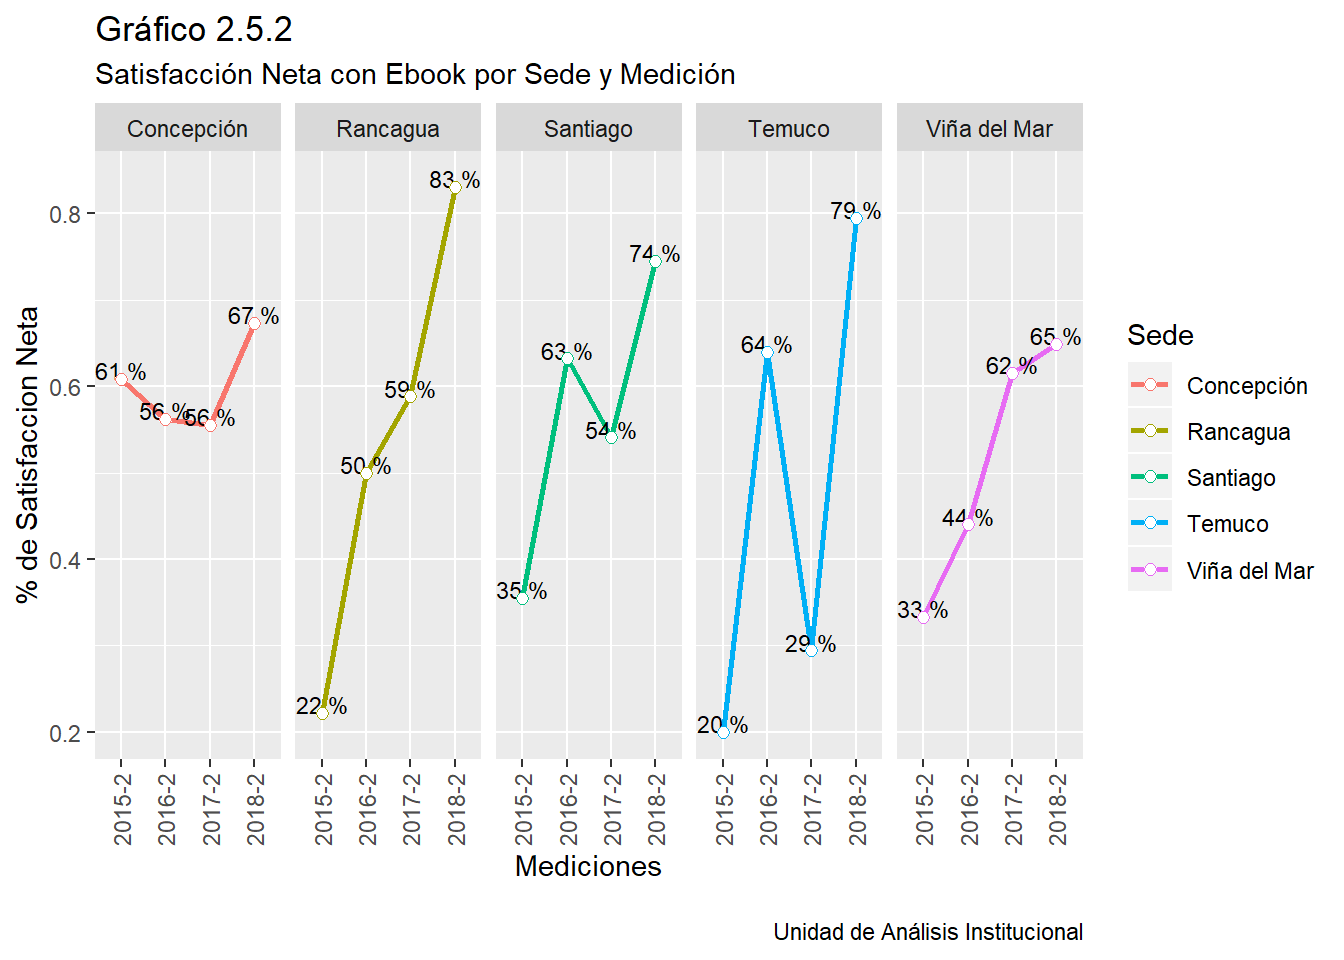
\includegraphics{bookdown_intro_files/figure-latex/unnamed-chunk-42-1.pdf}

** 2.3.5. Casino**

En un acápite anterior se observó que el espacio del Casino era aquella
que registraba una satisfacción neta más baja. El siguiente gráfico
permite adentrarse en dicha tendencia a nivel de cada una de las sedes.
El gráfico coincide con la sede con mejor a peor desempeño histórico. Se
puede apreciar que sólo \emph{Temuco} no registra una tendencia a la
baja desde el año 2017-2, incluso en el caso de \emph{Viña del Mar} se
registra un valor negativo (-26\%). Sólo en el caso de \emph{Temuco} se
aprecia una tendencia débil al alza, registrando un valor menos malo
(21\%) en la medición actual (2018-2).

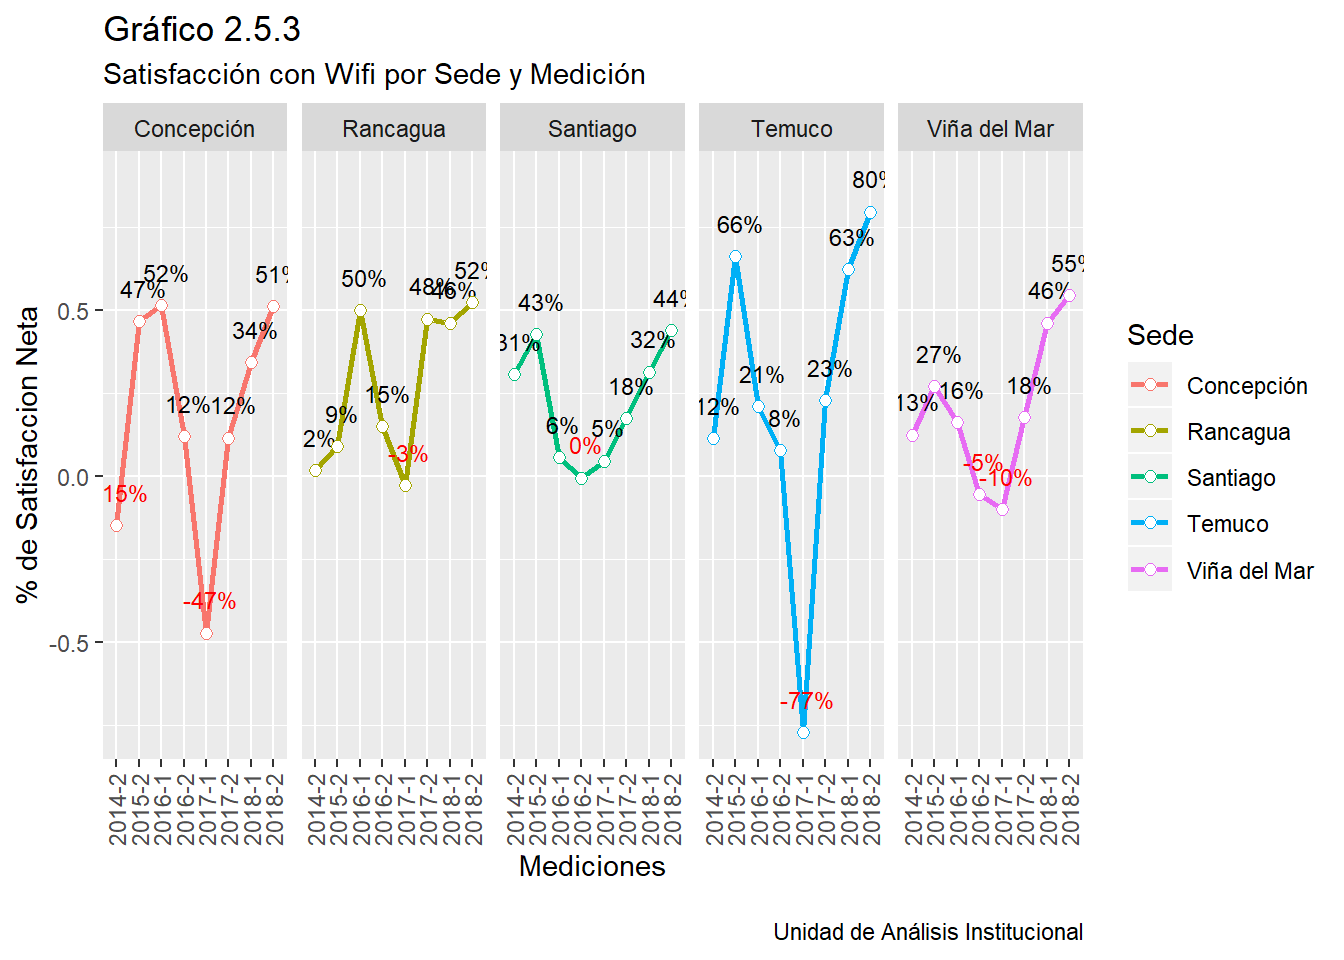
\includegraphics{bookdown_intro_files/figure-latex/unnamed-chunk-44-1.pdf}

** Jornada **

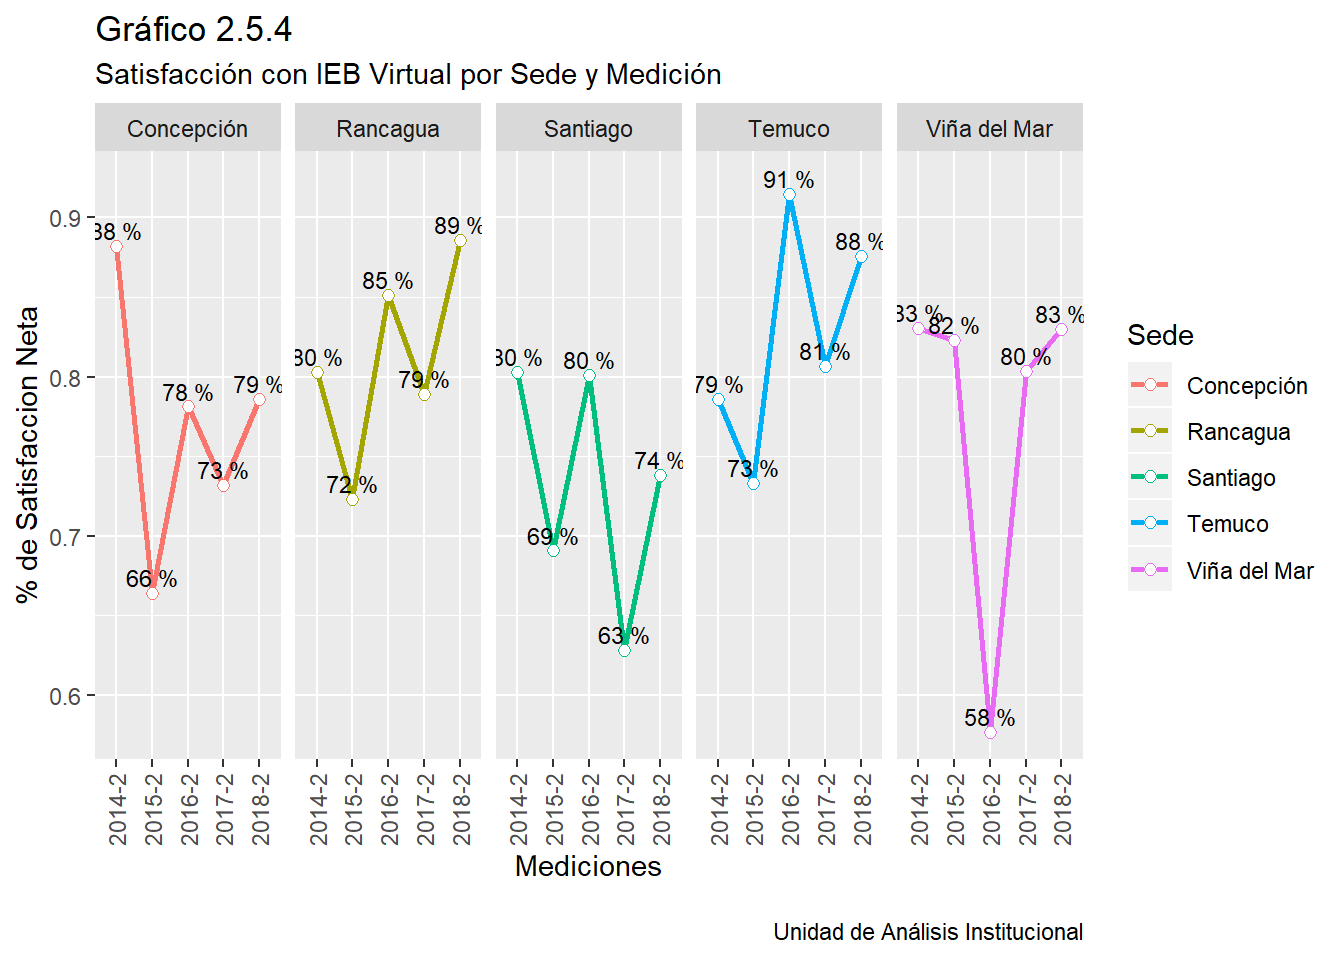
\includegraphics{bookdown_intro_files/figure-latex/unnamed-chunk-46-1.pdf}

\section{Satisfacción Neta con
Biblioteca}\label{satisfaccion-neta-con-biblioteca}

Anteriormente, se apreció que la \emph{Biblioteca} registra una alta
satisfacción neta en la presente medición (2018-2), en el gráfico
siguiente es posible apreciar cómo es esta tendencia en cada una de las
sedes. Se puede visualizar que existen caídas muy importantes en la
satisfacción neta en años puntuales según cada sede, exceptuando la sede
de \emph{Santiago} y \emph{Viña del Mar}. Más allá de estas caídas, ya
desde las mediciones del año 2017 existen incrementos que se han
mantenido en el tiempo, alcanzando en el caso de las sedes de
\emph{Rancagua}, \emph{Santiago} y \emph{Temuco}, valores en torno al
80\%.

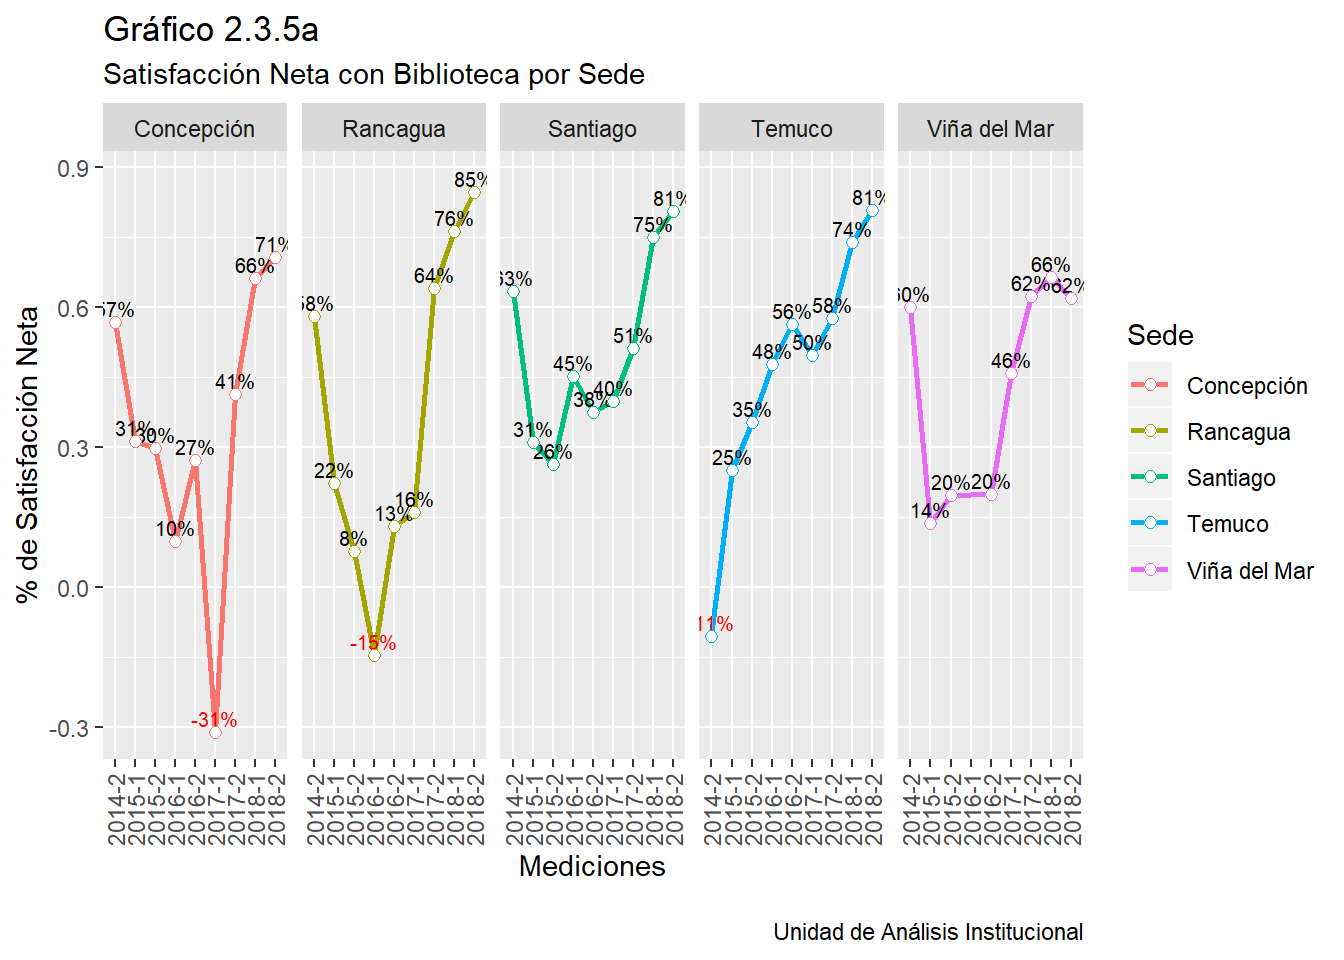
\includegraphics{bookdown_intro_files/figure-latex/unnamed-chunk-48-1.pdf}

** Jornada **

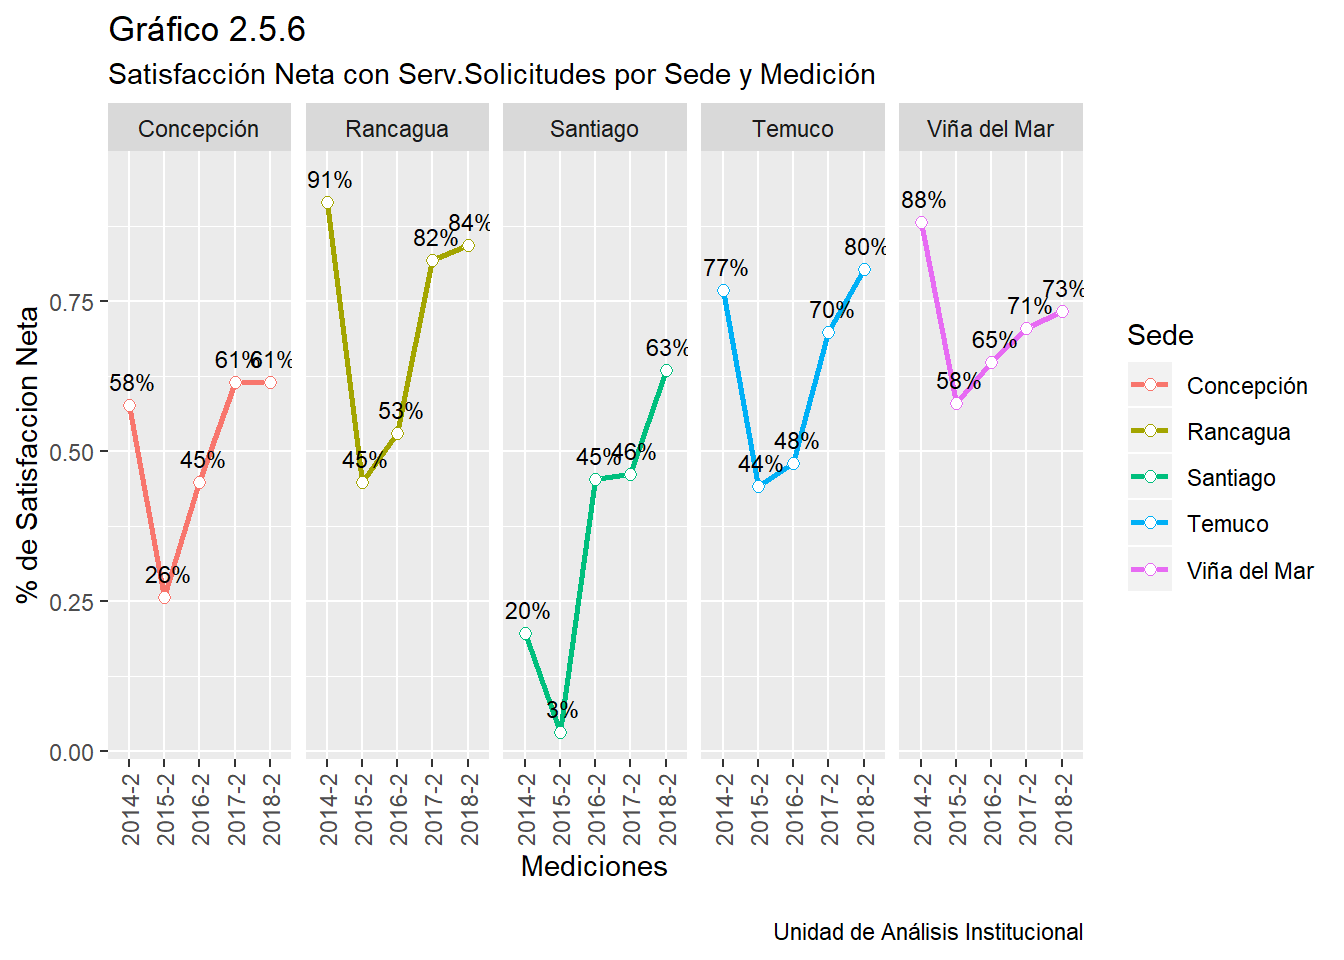
\includegraphics{bookdown_intro_files/figure-latex/unnamed-chunk-50-1.pdf}

En relación con la biblioteca, las sugerencias de mejoras de los
estudiantes corresponden principalmente a mejorar su
\textbf{Infraestructura}, esto queda reflejado de forma muy nítida en la
sede de \emph{Concepción} y \emph{Temuco}. A su vez, en la sede de
\emph{Rancagua} la petición se orienta a mejorar los \textbf{Horarios}
de funcionamiento.

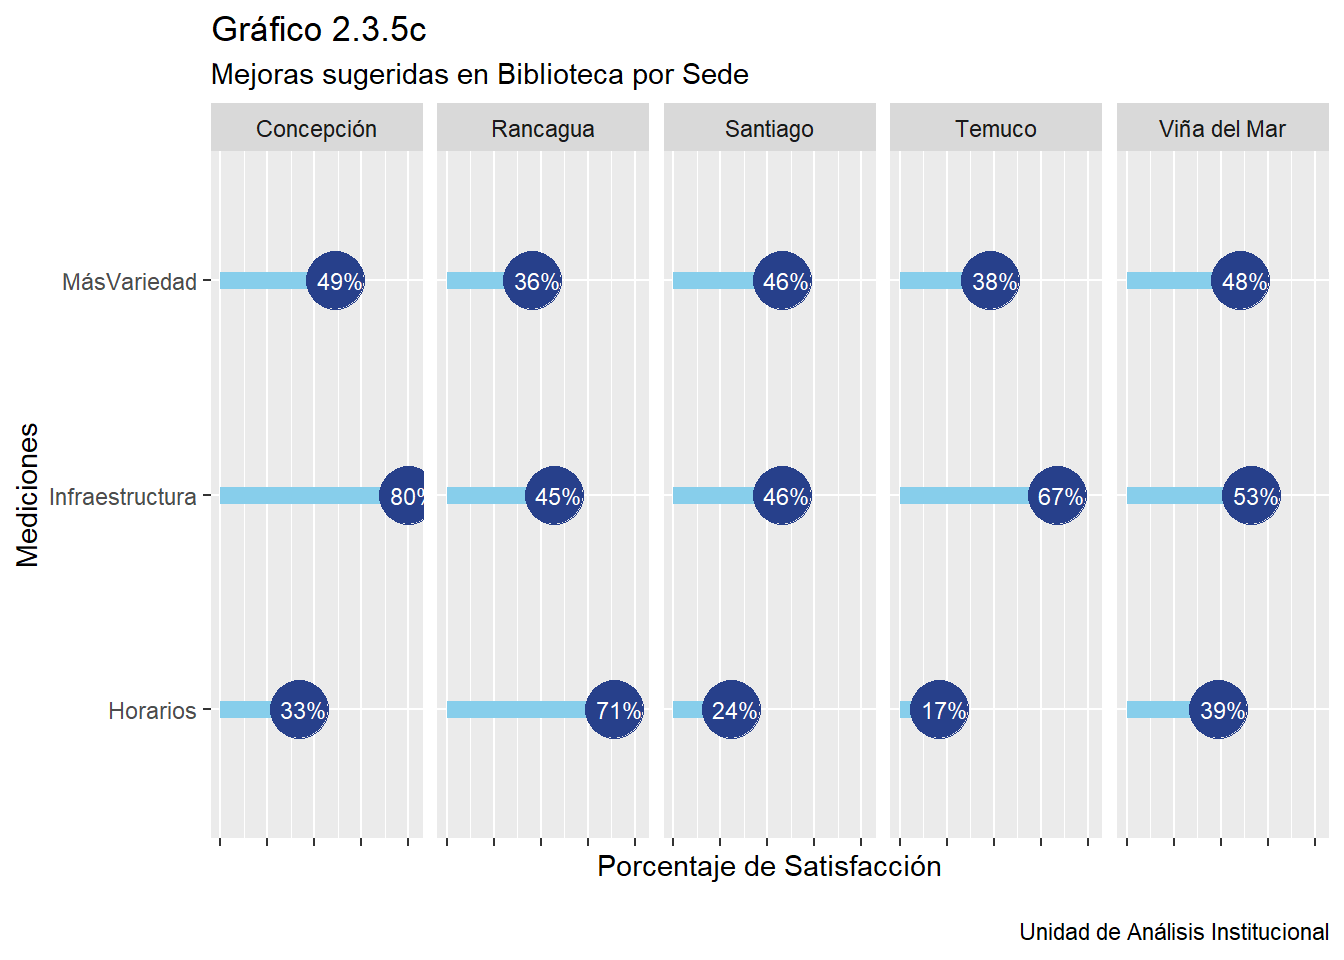
\includegraphics{bookdown_intro_files/figure-latex/unnamed-chunk-52-1.pdf}

\section{Satisfacción Neta con Espacios o Servicios
Digitales}\label{satisfaccion-neta-con-espacios-o-servicios-digitales}

Tres son los servicios o espacios que se han clasificado dentro de este
acápite: Plataforma IEB Virtual, Biblioteca Digital (Ebook) y Servicio
Wifi. El siguiente gráfico muestra los resultados obtenidos a nivel
histórico. Comparativamente se aprecia una mayor satisfacción respecto
de plataforma IEB Virtual, con valores que se mueven dentro de un mínimo
de 71\% y un máximo de 81\%. En segundo lugar, se puede apreciar la
valoración del Ebook (Biblioteca Digital), que en un inicio (2015-2)
alcanzaba los 36\%, en cambio ahora (2018-2) llega al 74\%. El servicio
Wifi genera una baja satisfacción neta, si bien ha remontado desde una
caída brusca en el año 2017-1, no supera en la medición actual el 54\%.

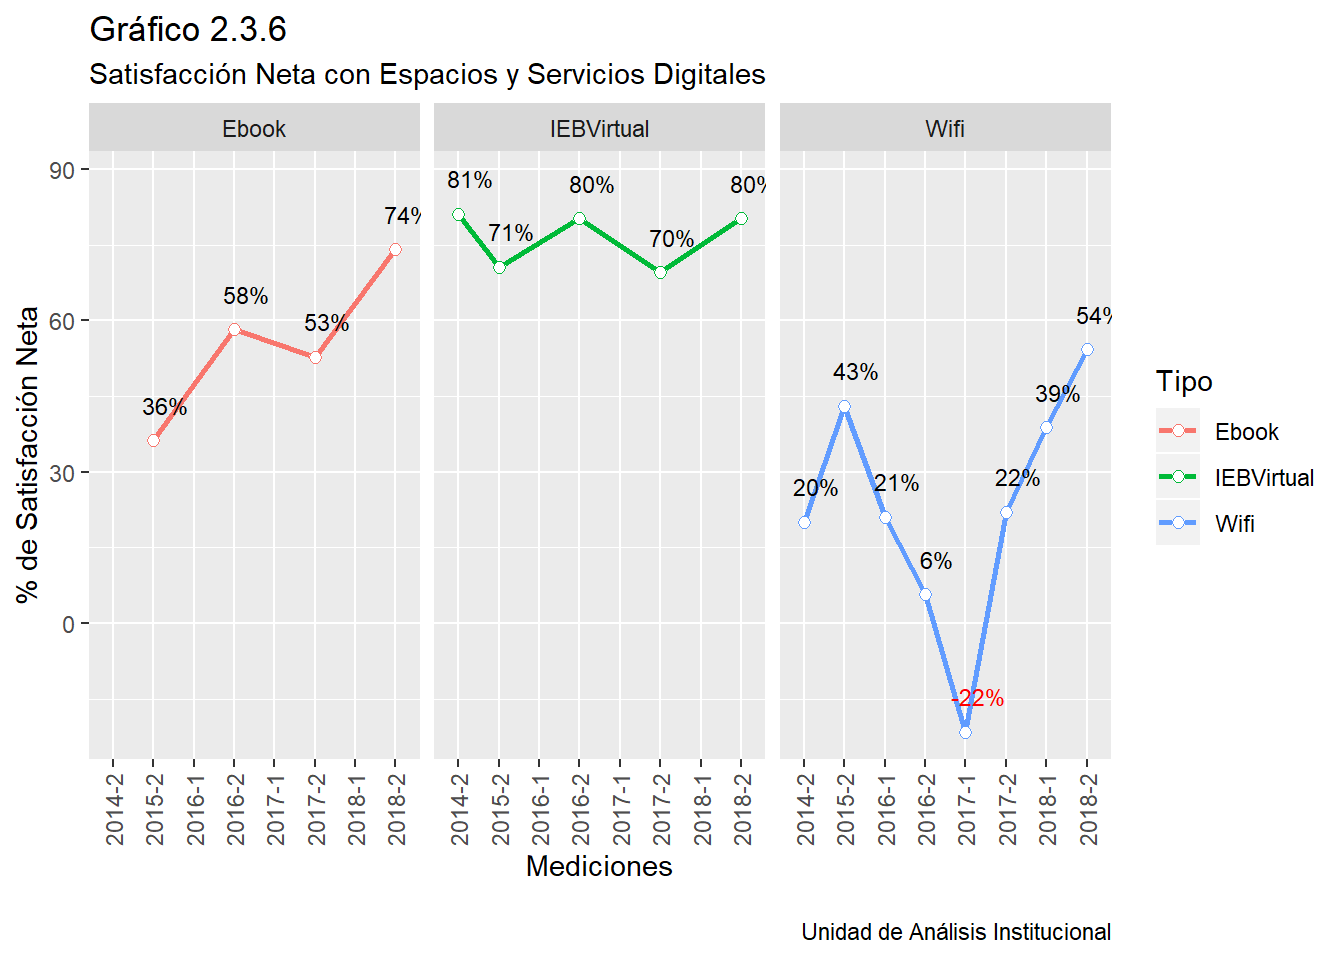
\includegraphics{bookdown_intro_files/figure-latex/unnamed-chunk-54-1.pdf}

** a) Ebook o Biblioteca Digital**

En la medición actual (2018-2), un \textbf{64\%} de los estudiantes
entrevistados indica haber utilizado el servicio de E-Books. A nivel de
cada sede, se visualiza que en \emph{Viña del Mar} y \emph{Concepción}
se registra una satisfacción menor. Por el contrario, la satisfacción,
al menos en 2018-2, es mayor en la sede de \emph{Rancagua} (83\%).

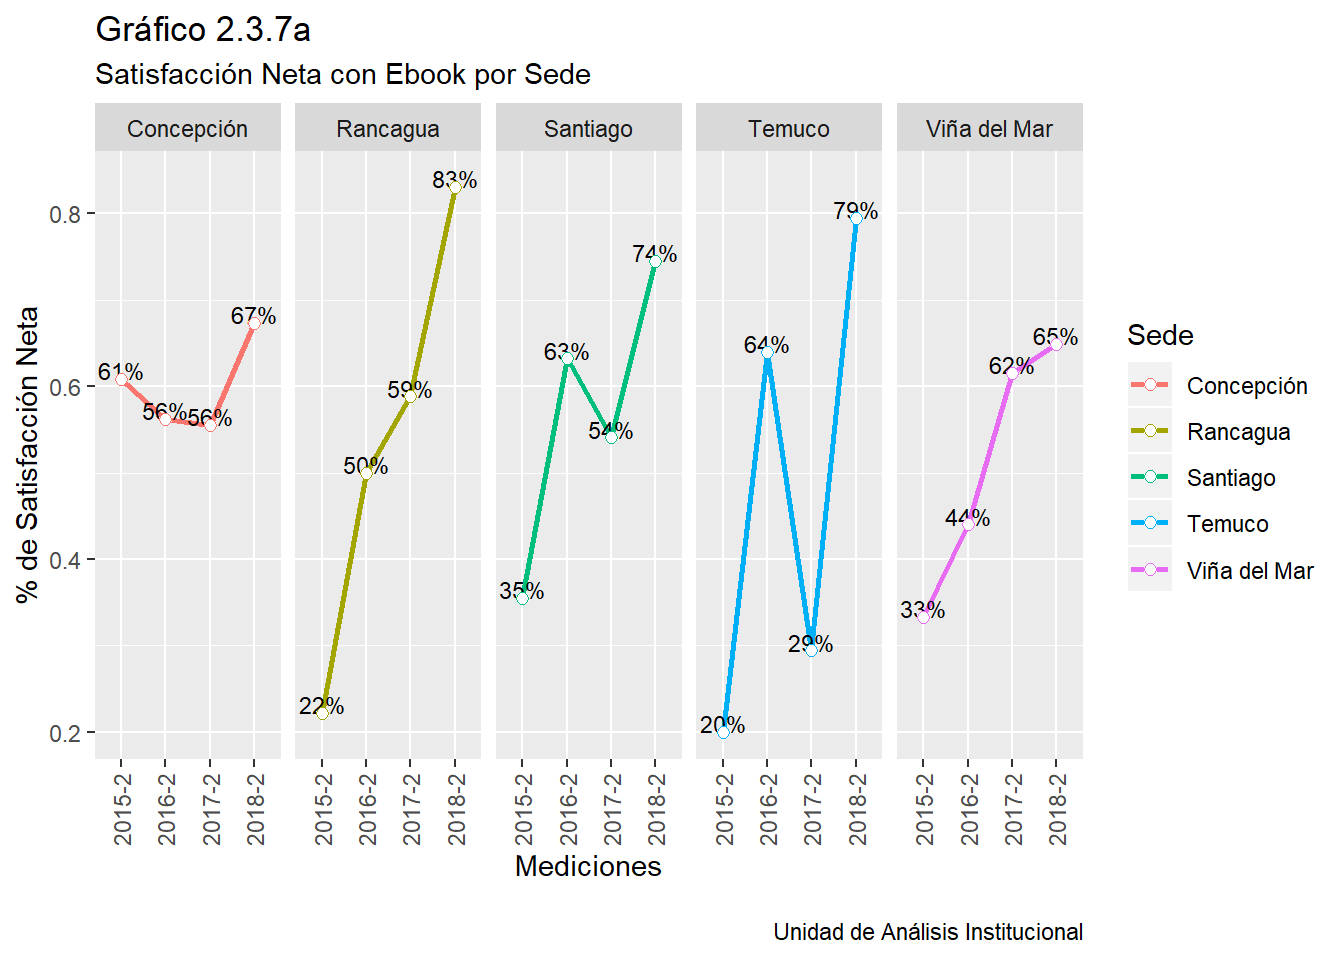
\includegraphics{bookdown_intro_files/figure-latex/unnamed-chunk-56-1.pdf}

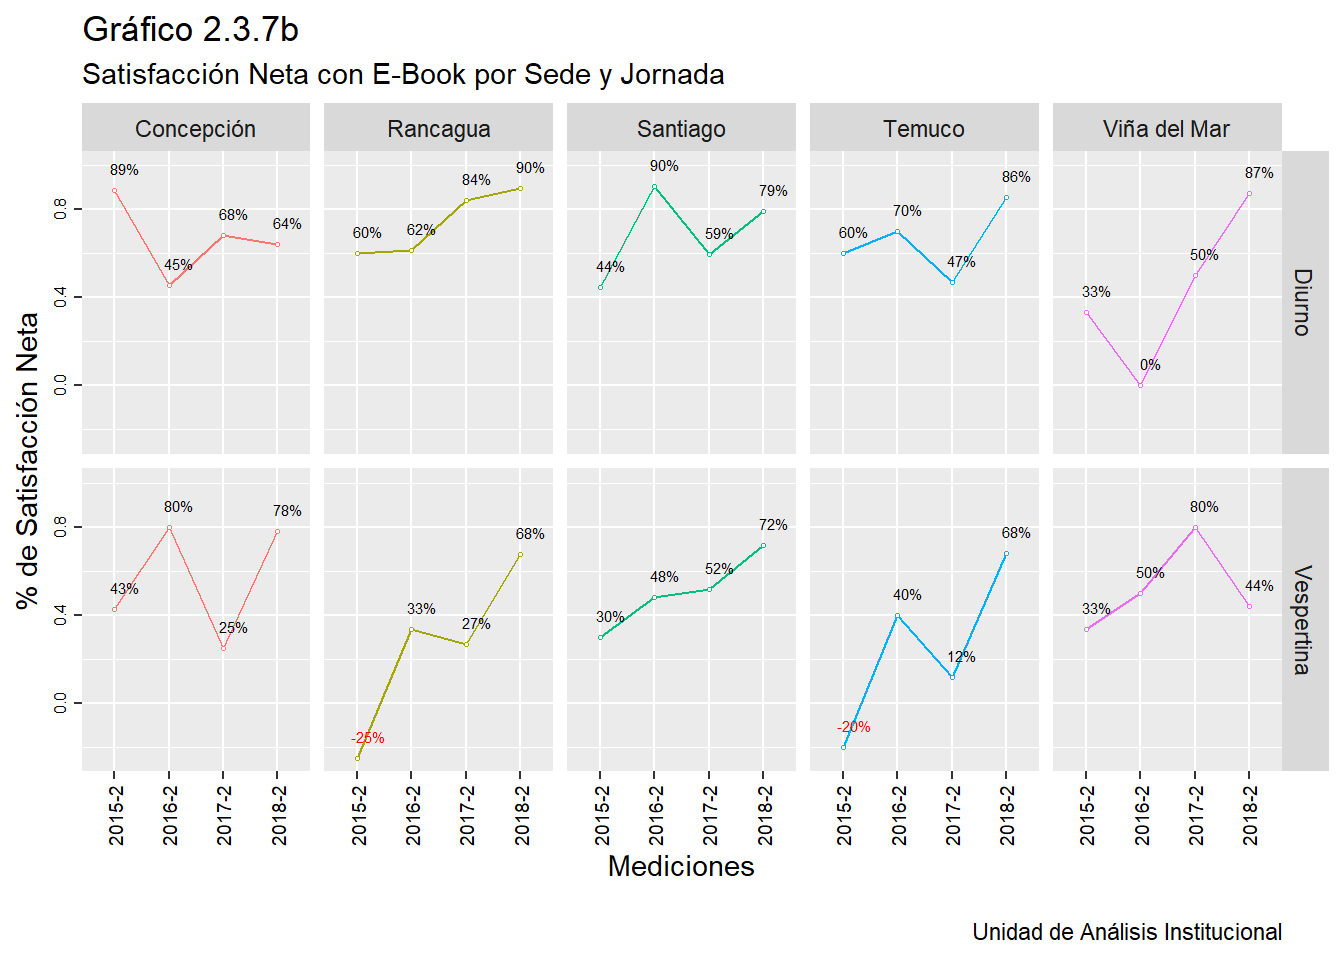
\includegraphics{bookdown_intro_files/figure-latex/unnamed-chunk-58-1.pdf}

** b) Servicio de Wifi**

El servicio se Wifi, o sea la posibilidad de los alumnos de acceder a
internet desde su laptop o celular en el mismo espacio físico de las
sedes, refleja una alta valoración en sus usuarios en la sede de
\emph{Temuco} (80\%), no obstante, en el resto de las sedes esta
satisfacción no supera el 55\%.

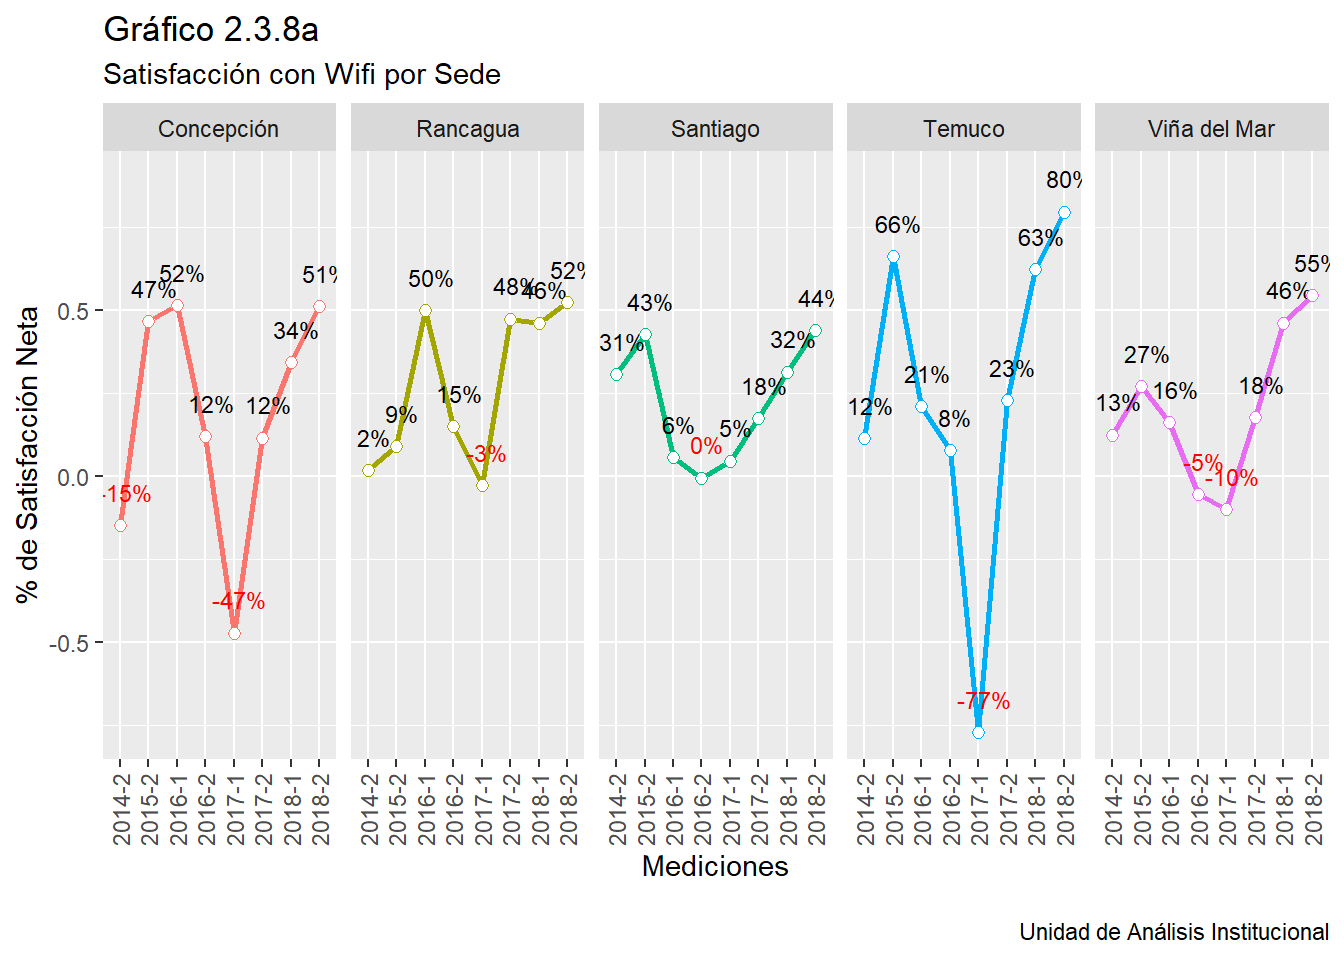
\includegraphics{bookdown_intro_files/figure-latex/unnamed-chunk-60-1.pdf}

** Jornada **

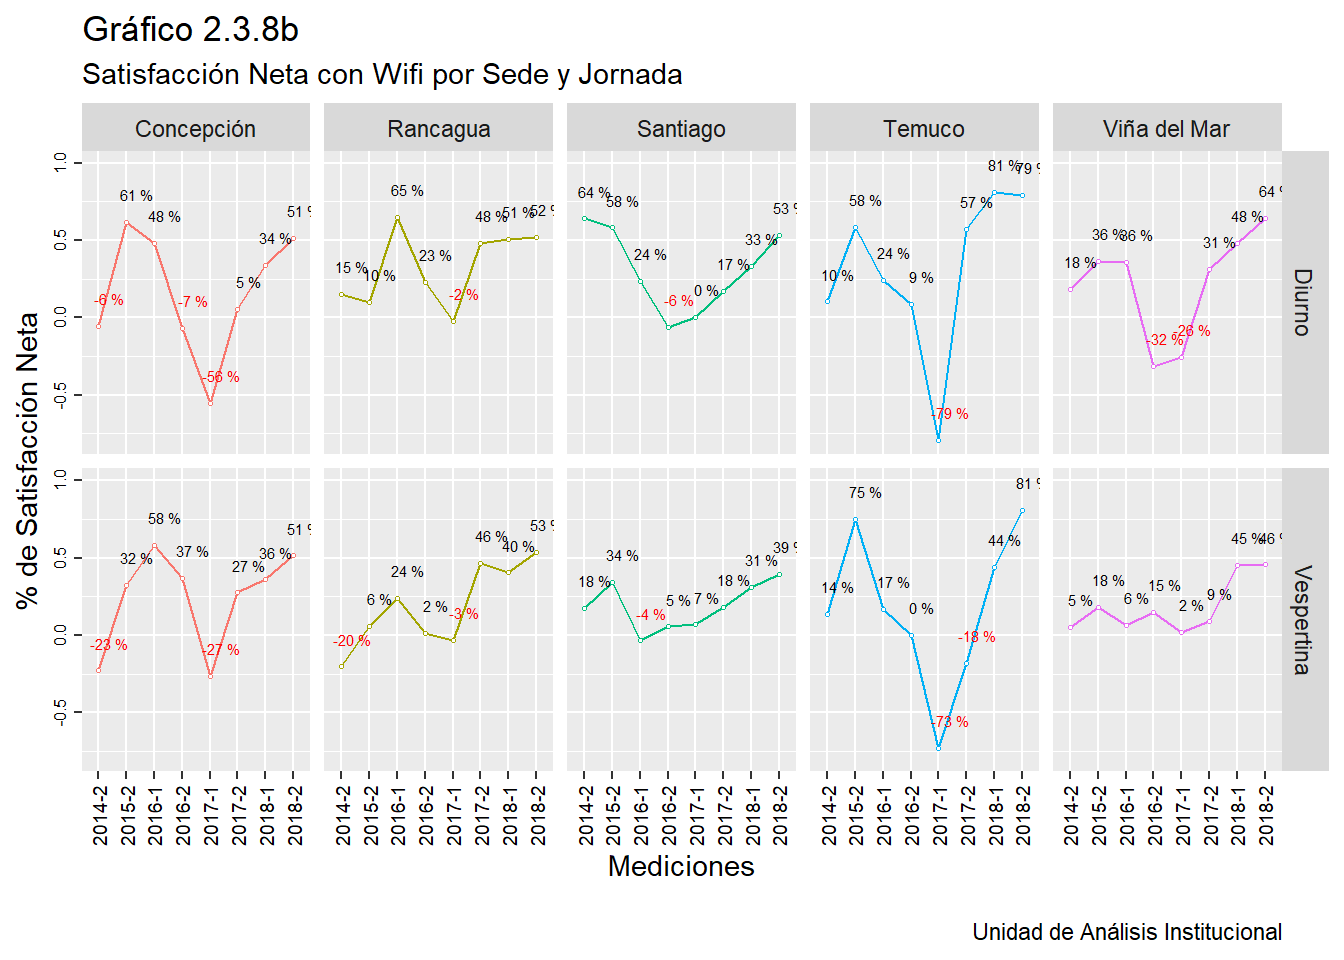
\includegraphics{bookdown_intro_files/figure-latex/unnamed-chunk-62-1.pdf}

** c) Plataforma IEB Virtual**

La satisfacción neta del IEB Virtual presenta la mejor evaluación dentro
de los servicios digitales evaluados. A nivel de cada sede, 4 de las 5
sedes alcanzan una satisfacción neta cercana al 80\%, mientras que en
\emph{Santiago} la satisfacción neta alcanza un 74\%.

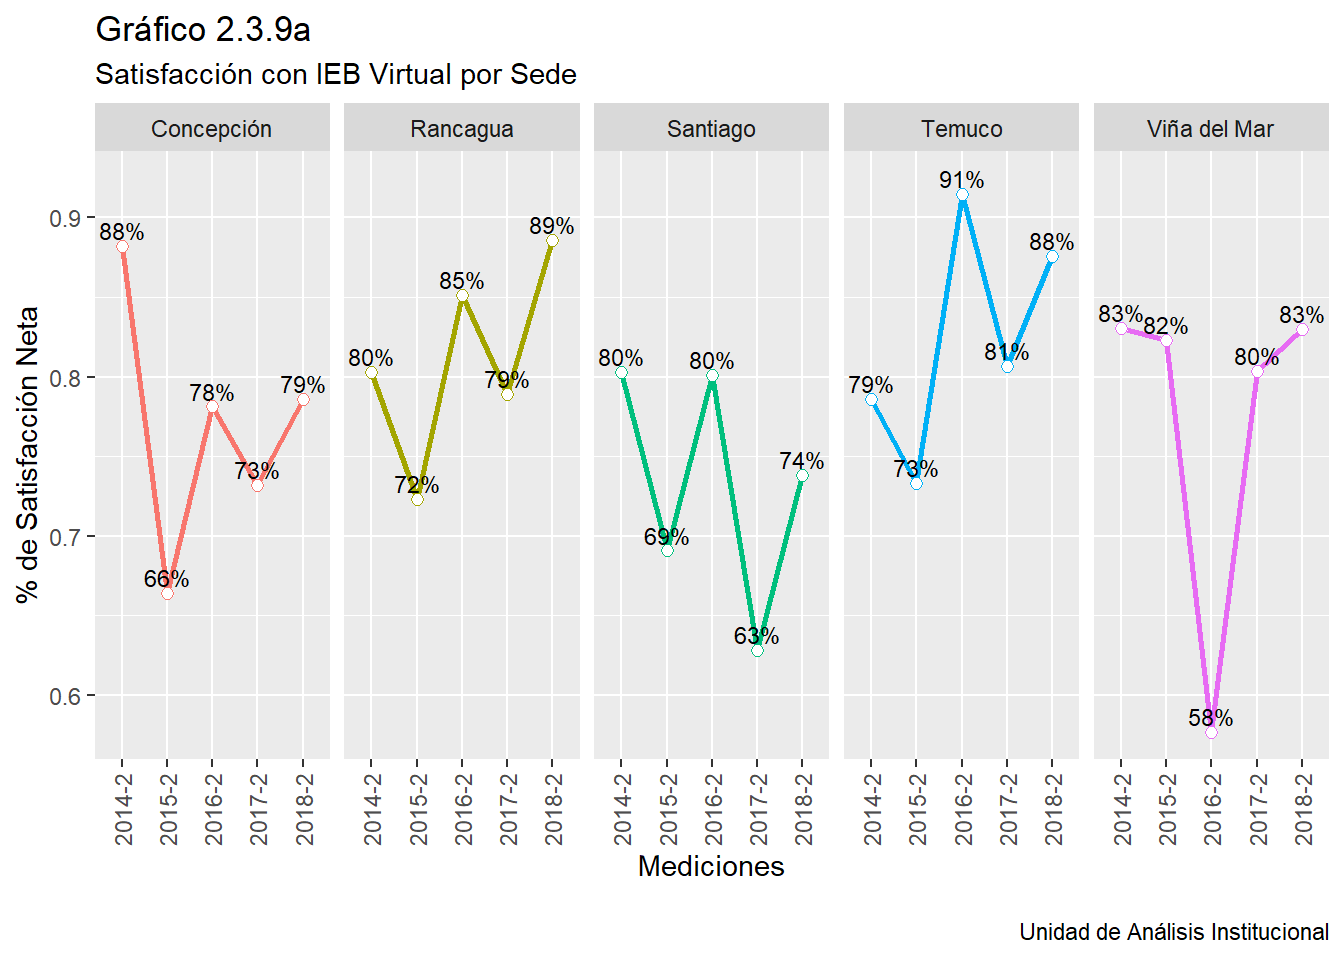
\includegraphics{bookdown_intro_files/figure-latex/unnamed-chunk-64-1.pdf}

** Jornada **

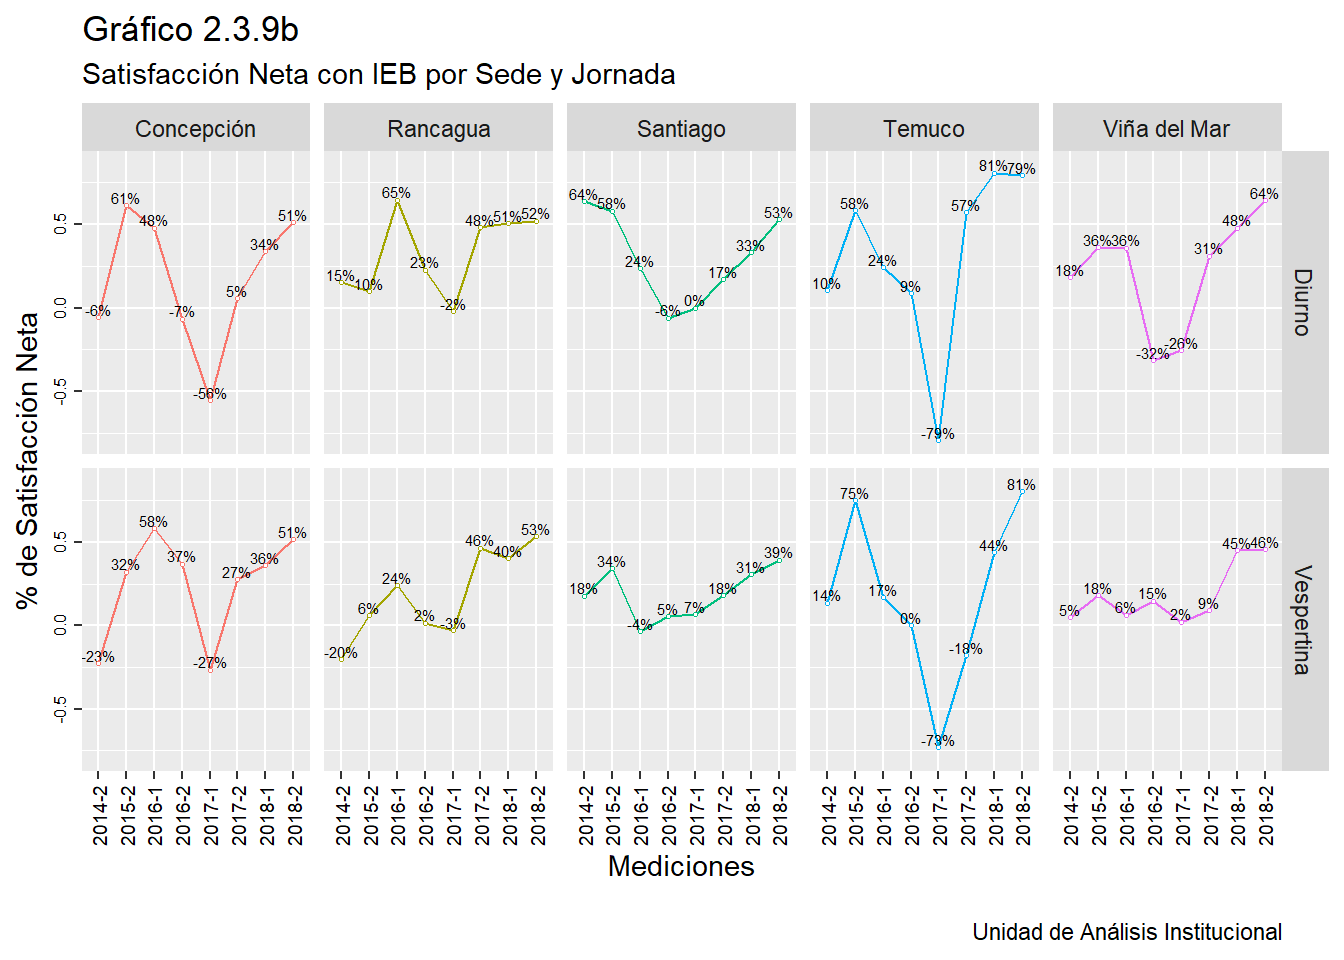
\includegraphics{bookdown_intro_files/figure-latex/unnamed-chunk-66-1.pdf}

\section{Satisfacción con Otros Servicios del
IGS}\label{satisfaccion-con-otros-servicios-del-igs}

En este acápite, por \emph{``otros servicios''}, se alude a Cajas y
Servicios de Solicitudes. En el primer aspecto, se ve una tendencia
clara hacia el alza desde el año 2015, llegando en el año 2018 a una
satisfacción neta de 71\%. En cuanto al servicio de solicitudes, su
tendencia es fluctuante, desde un valor inicial (2014-2) de 66\%,
bajando a un 22\% en el año 2016. En el año actual este servicio
registra un 61\% de satisfacción neta.

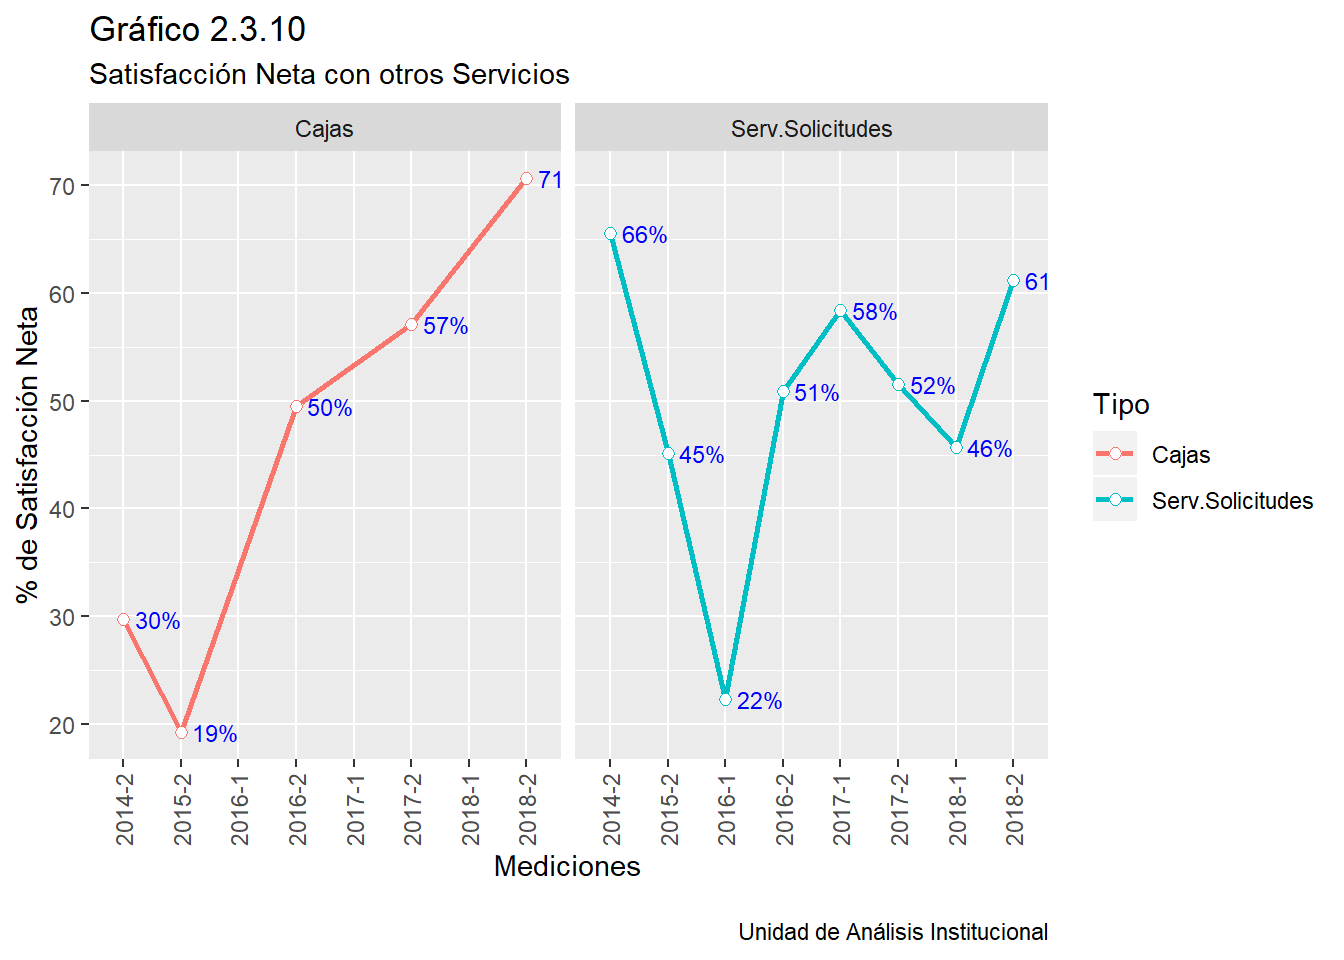
\includegraphics{bookdown_intro_files/figure-latex/unnamed-chunk-68-1.pdf}

** a) Servicio de Cajas**

Respecto del servicio de Caja por sede, se aprecia que en todas las
sedes hay una caída en el segundo año de medición. Sin embargo, desde
esa caída hay un repunte que se ha mantenido constante hasta la medición
actual. Los repuntes más altos, considerando de referencia la medición
actual, se registran en sede de \emph{Rancagua} y \emph{Temuco}. Más
leves son los repuntes registrados en las sedes de \emph{Concepción} y
\emph{Santiago}.

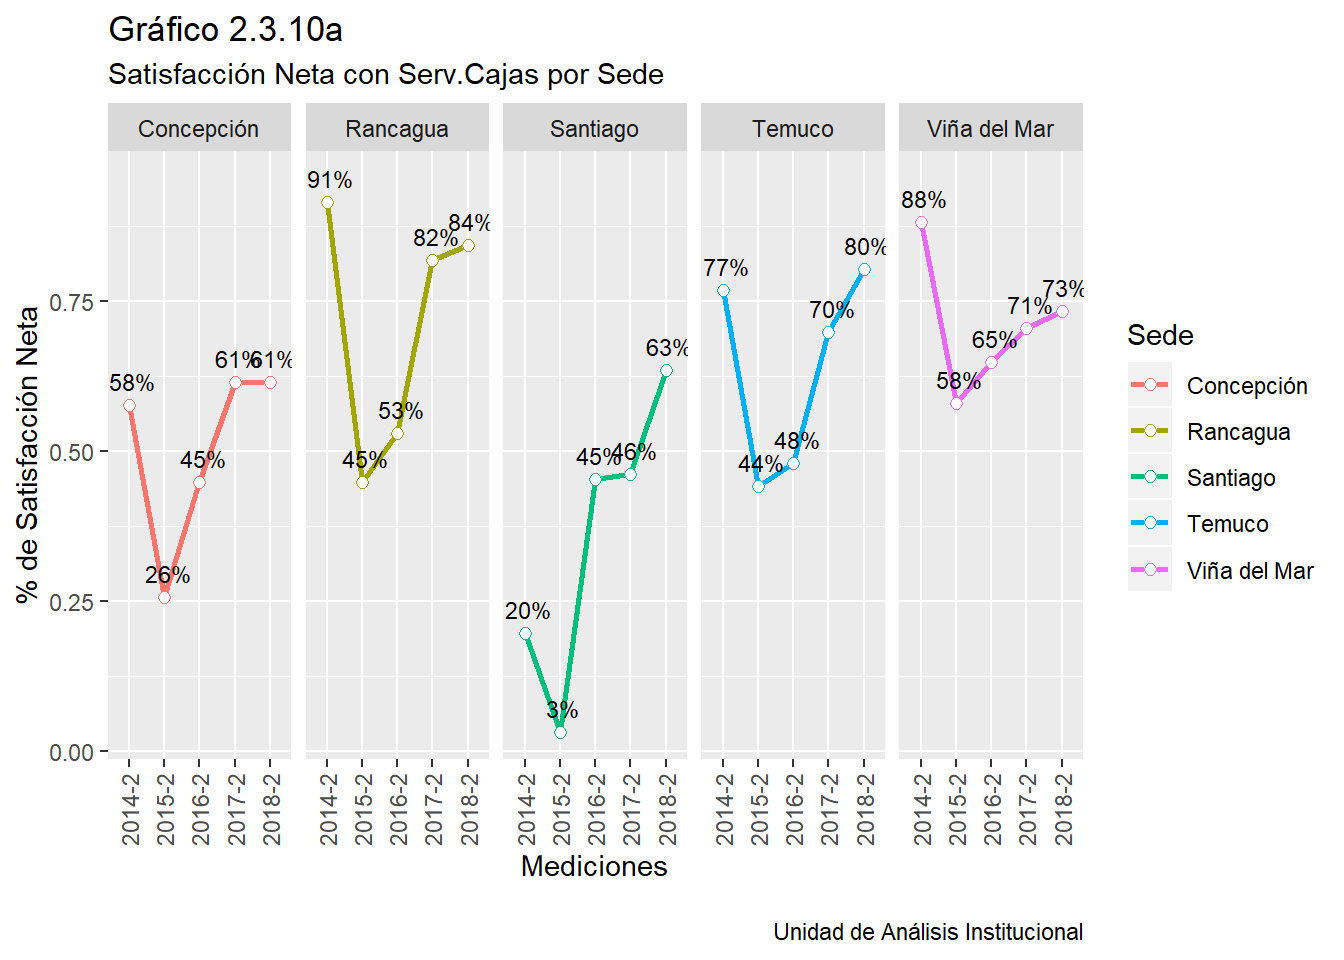
\includegraphics{bookdown_intro_files/figure-latex/unnamed-chunk-70-1.pdf}

** Jornada **

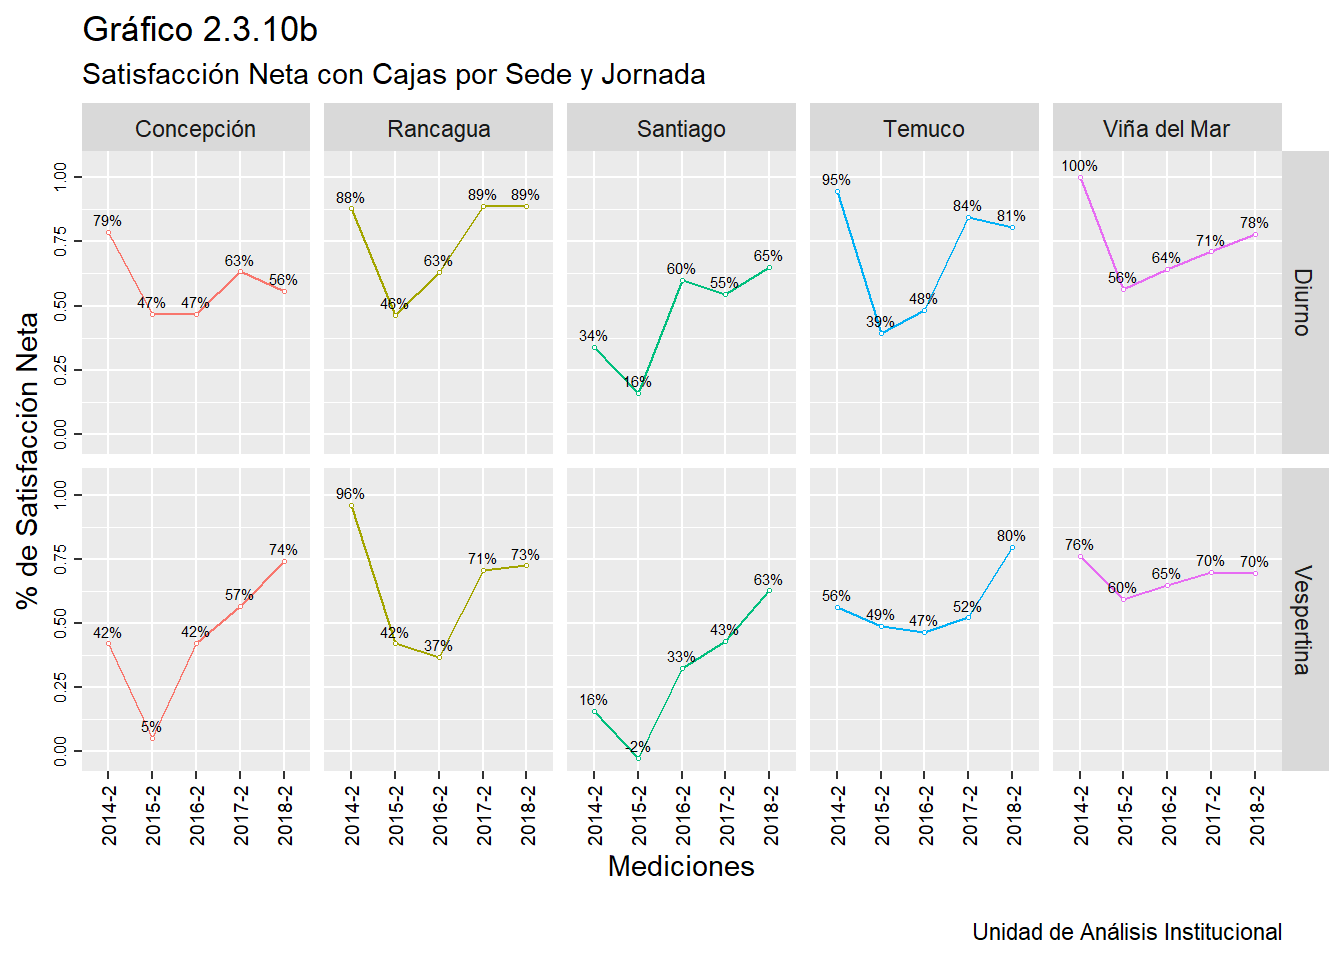
\includegraphics{bookdown_intro_files/figure-latex/unnamed-chunk-72-1.pdf}

** B) Servicio de Solicitudes**

El servicio de solicitudes tiene un comportamiento fluctuante en
términos de la satisfacción neta. Si se toma como referencia la última
medición (2018-2), se aprecia que todas las sedes mejoran respecto del
2018-1, destacándose la mejora en las sedes de \emph{Rancagua} y
\emph{Temuco}. Le siguen las sedes de \emph{Concepción} y \emph{Viña del
Mar}, por el contrario, se aprecia en la sede \emph{Santiago} un ascenso
leve de un 44\% de satisfacción neta.

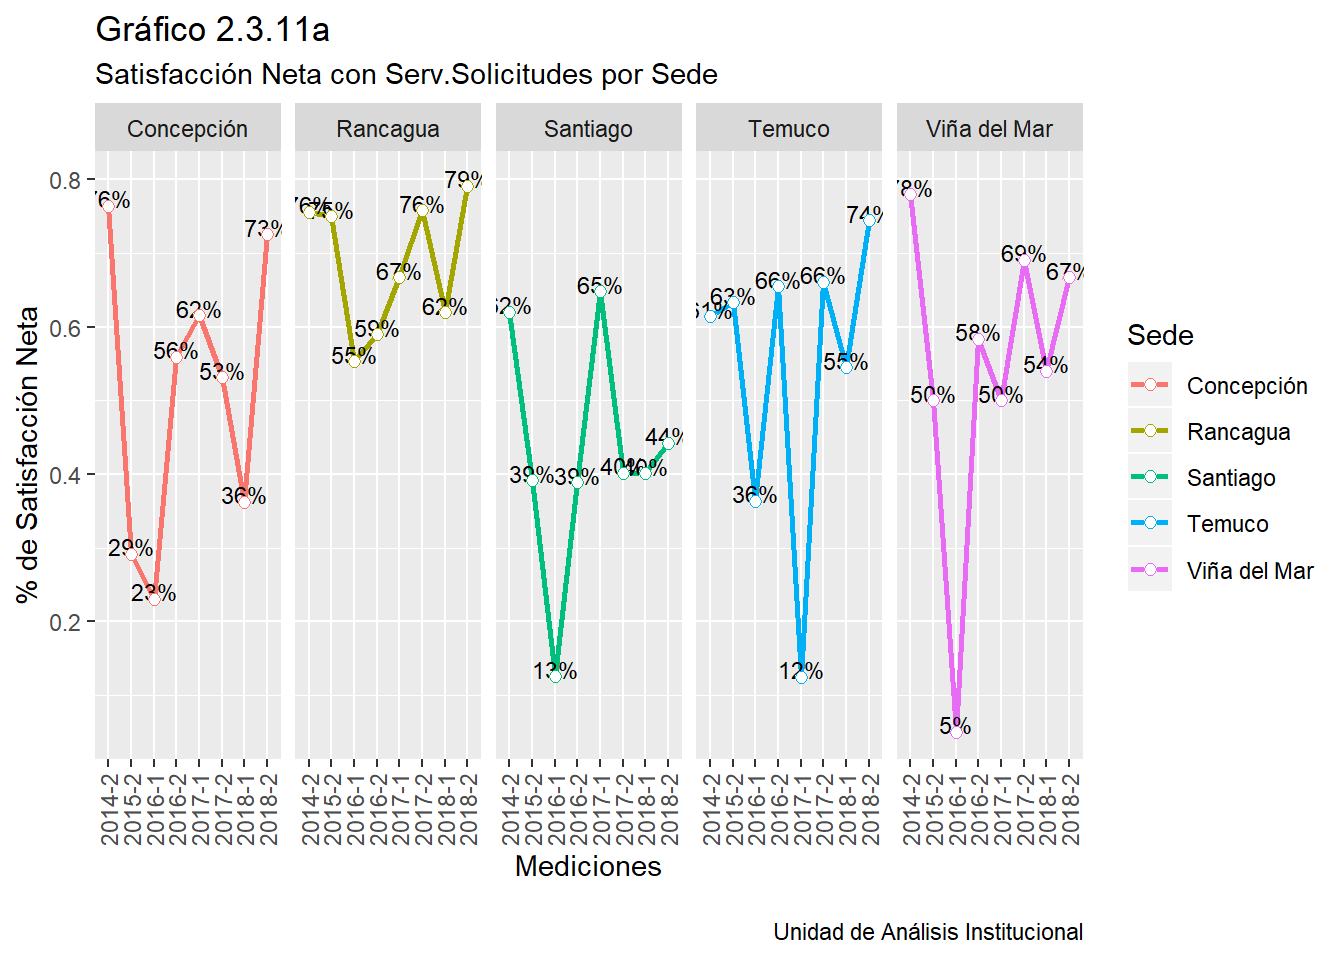
\includegraphics{bookdown_intro_files/figure-latex/unnamed-chunk-74-1.pdf}

** Jornada **

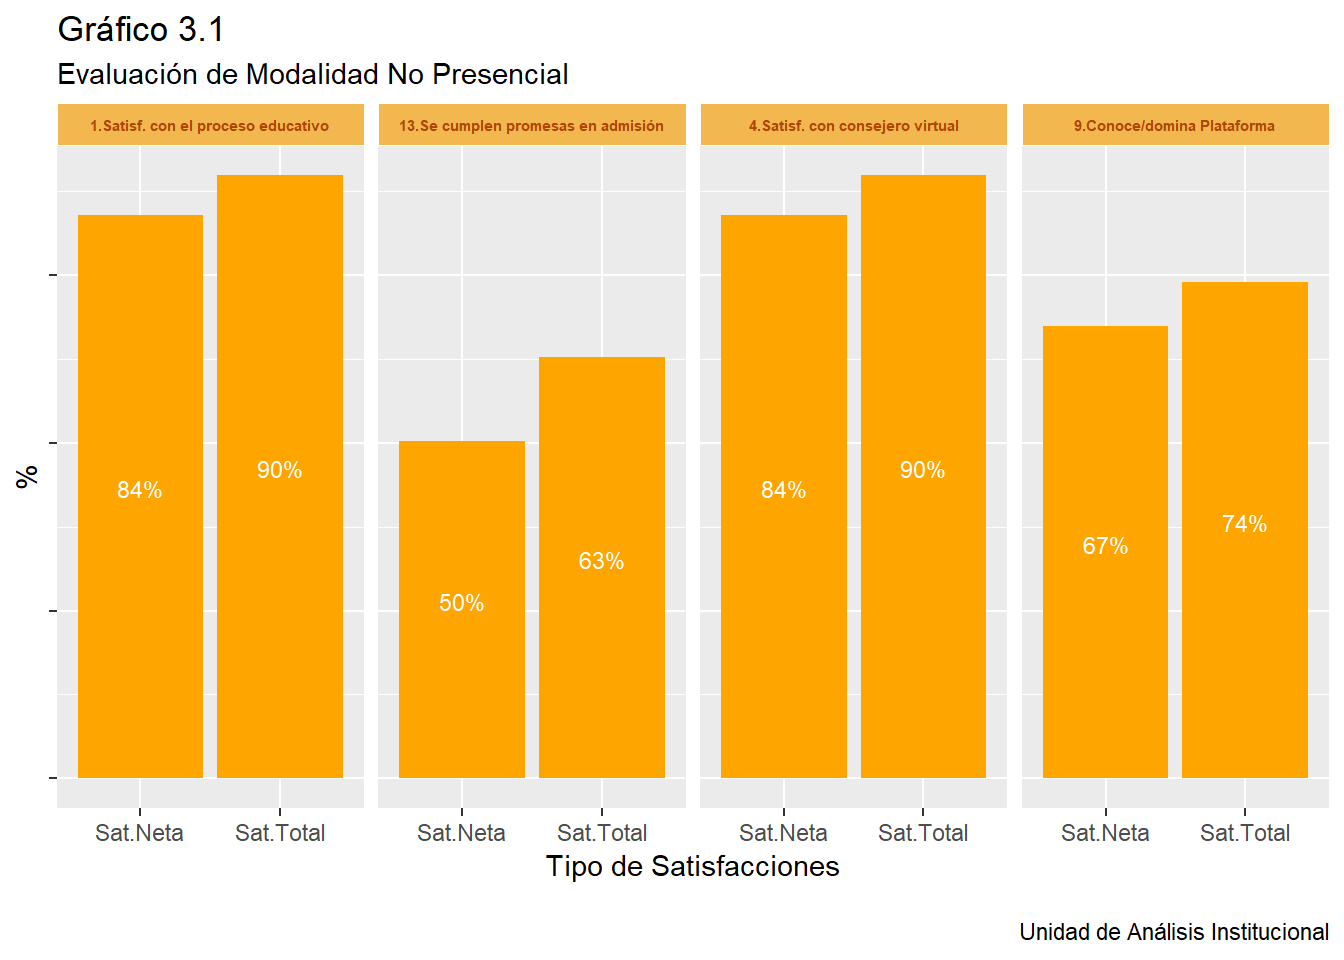
\includegraphics{bookdown_intro_files/figure-latex/unnamed-chunk-76-1.pdf}

\chapter{Análisis Multivariable}\label{analisis-multivariable}

\section{Regresión Logística}\label{regresion-logistica}

Con la finalidad de profundizar en los resultados obtenidos en la
encuesta de servicio 2018-2, se ha formulado dos modelos. El primer
modelo asume como variable dependiente la probabilidad de recomendar -o
no- el instituto a algún familiar o amigo; por otro lado, el segundo
modelo busca conocer cuáles son las variables significativas que hacen
más probable (o improbable) la evaluación con nota 6 ó 7 el servicio
entregado por el Instituto.

\begin{enumerate}
\def\labelenumi{\alph{enumi})}
\tightlist
\item
  Modelo Nº1: Probabilidad de recomendar el Instituto
\end{enumerate}

La disposición a recomendar el Instituto representa, en su base, es una
actitud condicionada por la experiencia que el estudiante ha tenido en
su rol de tal en un ciclo determinado. Por ende, se hace necesario
conocer cuáles, de las variables observadas, son factores que aumentan o
reducen la probabilidad de que el evento ocurra: el evento aquí es el
hecho de recomendar el Instituto.

Para responder al objetivo anterior, se ha hecho uso de la técnica
estadística de regresión logística multivariable. En el cuadro siguiente
se muestran algunos coeficientes que permiten aludir a la validez del
modelo.

Resumen del Modelo Nº1

\begin{longtable}[]{@{}lcc@{}}
\toprule
Log.de la verosimilitud -2 & R\textsuperscript{2} de Cox y Snell &
R\textsuperscript{2} de Negelkerke\tabularnewline
\midrule
\endhead
342,305 & 0,191 & 0,345\tabularnewline
\bottomrule
\end{longtable}

\begin{itemize}
\item
  \textbf{-2 log de la verosimilitud (-2LL)} mide hasta qué punto un
  modelo se ajusta bien a los datos. El resultado de esta medición
  recibe también el nombre de ``desviación''. El valor es moderado, lo
  ideal es que sea lo más bajo posible, por ello sólo se alude a un
  ajuste sólo aceptable.
\item
  \textbf{La R cuadradro de Cox y Snell} se utiliza para estimar la
  proporción de varianza de la variable dependiente explicada por las
  variables predictoras (independientes). La R cuadrado de Cox y Snell
  se basa en la comparación del log de la verosimilitud (LL) para el
  modelo respecto al log de la verosimilitud (LL) para un modelo de
  línea base. Sus valores oscilan entre 0 y 1. En nuestro caso es un
  valor moderado (0,191) que indica que sólo el 19\% de la variación de
  la variable dependiente es explicada por las variables incluidas en el
  modelo.
\item
  \textbf{La R cuadrado de Nagelkerke} es una versión corregida de la R
  cuadrado de Cox y Snell. La R cuadrado de Cox y Snell tiene un valor
  máximo inferior a 1, incluso para un modelo ``perfecto''. La R
  cuadrado de Nagelkerke corrige la escala del estadístico para cubrir
  el rango completo de 0 a 1. Aquí el valor alude a un modelo aceptable.
\end{itemize}

El siguiente cuadro muestra las variables significativas que son parte
del modelo.

\begin{center}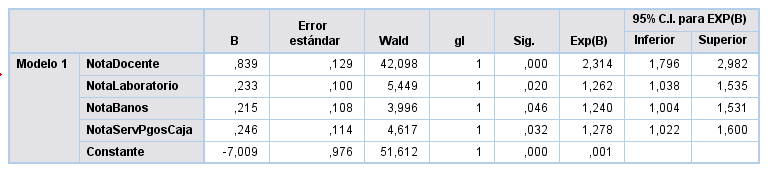
\includegraphics{images/Modelo1} \end{center}

La información del cuadro anterior, permite esbozar lo siguiente:

\begin{itemize}
\item
  Cada una de las variables contenidas en el cuadro han resultado ser
  significativas en términos estadístico, por ende, desempeñan un rol en
  relación a la ocurrencia del evento (recomendar).
\item
  Los valores de la columna b son positivos, lo que indica que cada una
  de las variables, al incrementarse en una unidad (en este caso de
  notas de 1 a 7), aumentan la probabilidad de ocurrencia del evento. Si
  el signo fuese negativo, indicaría que dicha variable desempeña un
  \emph{rol protector}, o sea, evita que ocurra el evento (recomendar el
  IGS).
\item
  El valor de la columna Exp(b) indica cuál de las variables
  seleccionadas tiene un mayor poder para explicar el evento de
  recomendar. En este contexto, este rol lo posee la variable nota a los
  docentes puesto que el valor de Exp(b) es el que más se aleja de 1,
  llegando a 2,314.
\item
  Si bien, como deja en claro el punto anterior, la evaluación de los
  docentes resulta ser clave en el hecho de recomendar o no el
  Instituto, están las otras variables las cuales aluden a espacios
  físicos de uso cotidiano para los alumnos, especialmente el área de
  servicios higiénicos y laboratorios. A su vez, aparece la evaluación
  de servicios de pago o cajas.
\end{itemize}

\begin{enumerate}
\def\labelenumi{\alph{enumi})}
\setcounter{enumi}{1}
\tightlist
\item
  Modelo Nº2: Probabilidad de Evaluar Servicios con Nota 6 o 7
\end{enumerate}

El Instituto define como satisfacción global las respuestas a la
pregunta ``\emph{evalúe la calidad de los servicios entregados por el
Instituto}''. En este aspecto, junto al modelo anterior, es necesario
conocer cuál de las variables observadas resulta ser factor en cuanto a
evaluar positiva o negativamente los servicios entregados por el
Instituto, o en otras palabras, que ocurra el evento de calificar con
nota 6 o 7 este tópico.

Al igual que en el modelo Nº1, se ha hecho uso de la técnica estadística
de regresión logística multivariable. En el cuadro siguiente se muestran
algunos coeficientes que permiten dar cuenta de la calidad estadística
del modelo.

Resumen del Modelo Nº2

\begin{longtable}[]{@{}lcc@{}}
\toprule
Log.de la verosimilitud -2 & R\textsuperscript{2} de Cox y Snell &
R\textsuperscript{2} de Negelkerke\tabularnewline
\midrule
\endhead
494,305 & 0,350 & 0,483\tabularnewline
\bottomrule
\end{longtable}

\begin{itemize}
\item
  \textbf{-2 log de la verosimilitud (-2LL)}. El valor de este
  coeficiente es moderado, lo ideal es que sea lo más bajo posible, por
  ello sólo se alude a una calidad del modelo aceptable.
\item
  \textbf{La R cuadrado de Cox y Snell}. Los valores de este coeficiente
  oscilan entre 0 y 1. En este caso el valor es moderado (0,350), lo que
  indica que el 35\% de la variación de la variable dependiente es
  explicada por las variables incluidas en el modelo.
\item
  \textbf{La R cuadrado de Nagelkerke}. El valor de este coeficiente da
  cuenta de un modelo aceptable.
\end{itemize}

El siguiente cuadro muestra las variables significativas que son parte
del modelo.

\begin{center}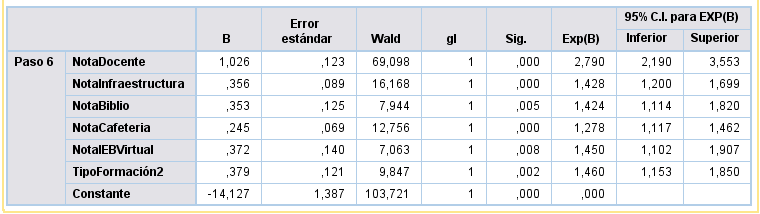
\includegraphics{images/Modelo2} \end{center}

La información del cuadro anterior, permite esbozar lo siguiente:

\begin{itemize}
\item
  Cada una de las variables contenidas en el cuadro desempeñan un rol
  estadístico en relación a la ocurrencia del evento (recomendar).
\item
  Los valores de la columna b son positivos, lo que indica que al
  aumentar cada una de las variables aumentan también la probabilidad de
  ocurrencia del evento (calificar con nota 6 y 7 el servicio entregado
  por el Instituto). Si el signo fuese negativo, indicaría que dicha
  variable desempeña un \emph{rol protector}, o sea, evita que ocurra el
  evento.
\item
  El valor de la columna Exp(b) indica cuál de las variables
  seleccionadas tiene un mayor poder para explicar el evento de
  recomendar. En este contexto, al igual como ocurre en el modelo nº1,
  este rol lo posee la variable ``NotaDocentes'', donde el valor de
  Exp(b) es el más alto, llegando a 2,190.
\item
  En este modelo, aparecen relevantes 3 variables relacionadas con el
  aspecto material-espacial del Instituto (Infraestructura, Biblioteca y
  Cafetería), una de espacio virtual (IEB-Virtual). Estas variables
  indican que a medida que aumenta en una unidad la calificación (de
  nota 1 a 7), aumenta la probabilidad que el estudiante evalúe con nota
  6 ó 7 el servicio entregado por el Instituto. Una última variable se
  relaciona con el perfil del estudiante (técnico versus profesional);
  en este caso cuando el estudiante pasa de técnico a profesional
  aumenta la probabilidad de evaluar con nota 6 ó 7 al Instituto en
  cuanto al servicio que entrega.
\end{itemize}

\chapter{Conclusiones}\label{conclusiones}

\begin{itemize}
\item
  En materia de percepción general, se aprecia que en el año actual la
  satisfacción neta con los \textbf{servicios entregados} alcanza 51\%,
  así como en \textbf{calidad de la atención} se alcanza el 63\%. En
  ambos casos, este dato es superior a las últimas mediciones
  realizadas. A nivel de sedes, se aprecia que el desempeño del primer
  indicador es superio en las sedes de Temuco(67\%) y Viña del
  Mar(65\%), por el contrario, resultó más bajo en Santiago (36\%) y
  Concepción (52\%). En cuanto a la Calidad de la atención, también
  resulta alto en Rancagua (80\%) y Viña del Mar (79\%), el más bajo es
  Santiago (46\%). Si bien en esta última sede es bajo, el valor ha
  venido de forma sostenda mejorando.
\item
  En materia de percepción general, sobresale la disposición positiva
  por recomendar el instituto, así se alcanzó que un 46\% dice que
  probablemente sí lo haría, y un 40\%, dice que \emph{definitivamente}
  sí lo haría. Esta última categoría no deja dudas respecto de la
  satisfacción positiva con el instituto, y su valor alcanzado en
  2018-2(40\%), es superior a los años anteriores.
\item
  Otro aspecto clave de evaluar corresponde a los \textbf{Docentes}. En
  este ámbito, se aprecia que la satisfacción neta alcanza un 64\% en
  2018-2. Este valor es superior en 9 puntos respecto de la medición
  anterior (55\%).A nivel de Sede, destaca el valor 2018-2 que se
  registra en Rancagua y Temuco, ambos con 79\%. El valor es más bajo en
  Concepción (71\%) y Santiago (49\%).
\item
  En cuanto a los servicios asociados con \textbf{espacios físicos}, se
  aprecia que el desempeño del espacio de \emph{biblioteca} (física) ha
  mejorado su desempeño desde la medición de 2017-1, incluso en 2018-1
  supera en más de 10 puntos a los otros espacios de atención. Por el
  contrario, el \emph{casino/cafetería} es el espacio con una menor
  magnitud de satisfacción neta, tanto a nivel histórico como en cada
  una de las sedes. Incluso, en este mismo ámbito, se constata una baja
  desde 2017-2 a 2018-2, pasando del 25\% al 14\%.
\item
  En cuanto a los \textbf{servicios digitales o virtuales}, se puede
  apreciar que \emph{Ebook} (biblioteca virtual) ha venido mejorando
  medición tras medición, llegando en la última mediicón a 74\%. Por
  otra parte, los estudiantes tienen una percepción positiva de
  \emph{IEB Virtual}, así la satisfacción neta no baja del 70\%. En este
  ámbito, el servicio de \emph{WIFI} es aquel que tiene una evaluación
  más negativa, especialmente en la medición 2017-1 éste valor es
  negativo (-22\%), ahora bien, este indicador ha mejorado desde dicha
  medición, alcanzando en la última medición los 54\% puntos
  porcentuales.
\item
  En relación con servicios como \textbf{cajas}, se puede apreciar que
  éste ámbito ha venido mejorando en la percpecion de los estudiantes.
  De esta forma, en la medición de 2015-2 alcanza el 19\%, pero ya desde
  ese punto se genera un punto de inflexión al alza que se sostiene y
  llega en 2018-2 al 71\% en la última medición. Otro servicio evaluado,
  corresponde al \textbf{servicio de solicitudes}, servicio que es
  evaluado de forma irregular en el tiempo, tendiendo a una baja
  significativa en la medición 2016-1, de ahí sube en 2017-1 a 58\%,
  pero desciende nuevamente en 2018-1 (46\%) y vuelve a subir en 2018-2
  a 61\%.
\end{itemize}

\appendix


\chapter{Anexo 2}\label{rmarkdown}

Anexo 1 \{\#pandoc\}

\bibliography{book.bib,packages.bib}


\end{document}
